\documentclass[../midgard.tex]{subfiles}
\graphicspath{{\subfix{../images/}}}
\begin{document}

\def\txDiagramScale{0.9}

\chapter{Midgard L1 transactions}
\label{h:midgard-l1-tx}

This chapter specifies the L1 transactions that interact with Midgard's consensus protocol smart contracts.
Whereas the onchain smart contract are specified in a modular way, where each validator is only concerned with its own validity conditions, the transactions specified in this chapter often interact with several of the onchain validators and must satisfy all of their conditions.
Thus, the offchain code can be seen as the integration layer for the onchain code.

\begin{figure}[H]
\begin{center}
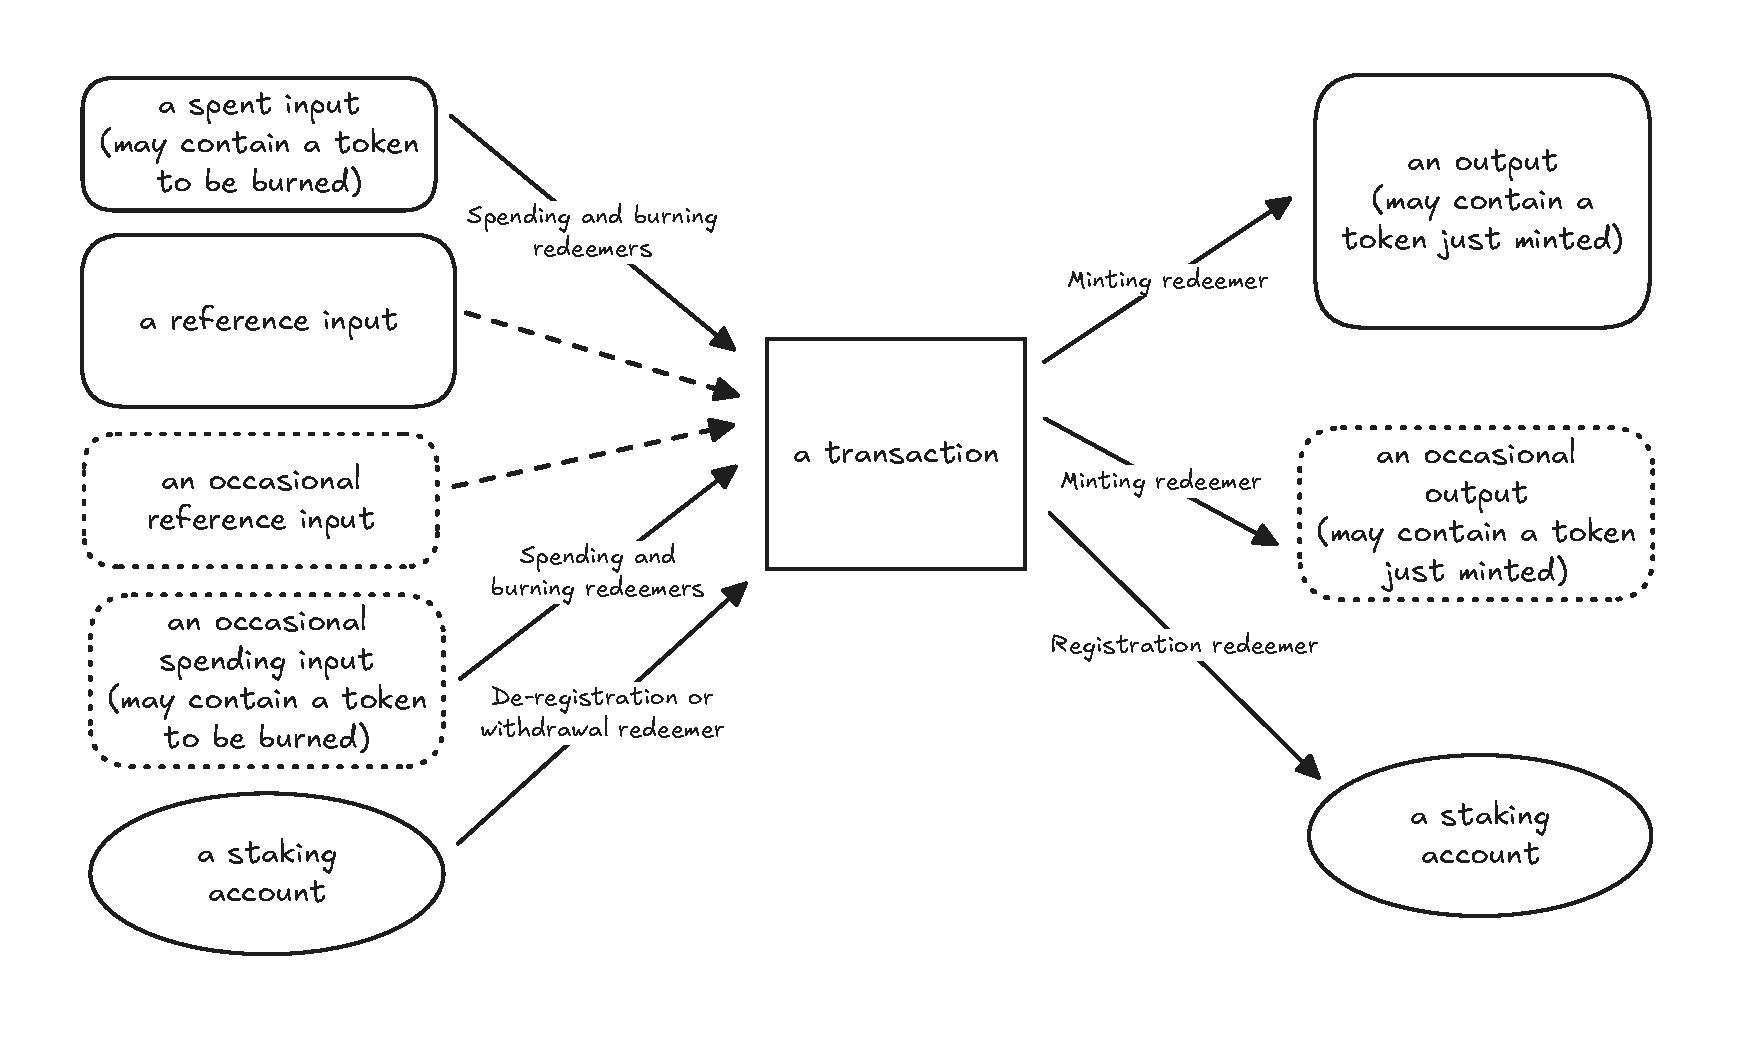
\includegraphics[width=\txDiagramScale\linewidth]{\subfix{../images/tx-diagram/Z-example-diagram.pdf}}
\end{center}
\caption[Example transaction diagram]{Example transaction diagram.}
\label{fig:tx-example}
\end{figure}

As illustrated in the example diagram (\cref{fig:tx-example}), interpret our transaction diagrams as follows:
\begin{itemize}
  \item Transactions are sharp-corner rectangles.
  \item Spent inputs are rounded-corner rectangles with outgoing arrows to transactions.
  \item Reference inputs are rounded-corner rectangles with dashed outgoing arrows to transactions.
  \item Outputs are rounded-corner rectangles with incoming arrows from transactions.
  \item Staking account are ellipses with incoming arrows from transactions if they're being registered and outgoing arrows to transactions if they're being de-registered or withdrawn from.
  \item Occasional inputs/outputs are rounded-corner rectangles with dotted borders. This indicates that these inputs/outputs may sometimes be present in transactions, but may be absent in other times.
  \item Spending redeemers label arrows from inputs to transactions.
  \item Burning redeemers label arrows from inputs to transactions, when those inputs contain tokens to be burned by the transactions.
  \item Minting redeemers label arrows from transactions to outputs, when those outputs contain tokens minted by the transactions.
  \item Redeemer labels may be omitted when scripts have only one possible redeemer.
\end{itemize}

\section{Initialization}%
\label{h:midgard-l1-tx-initialization}%

\begin{figure}[H]
\begin{center}
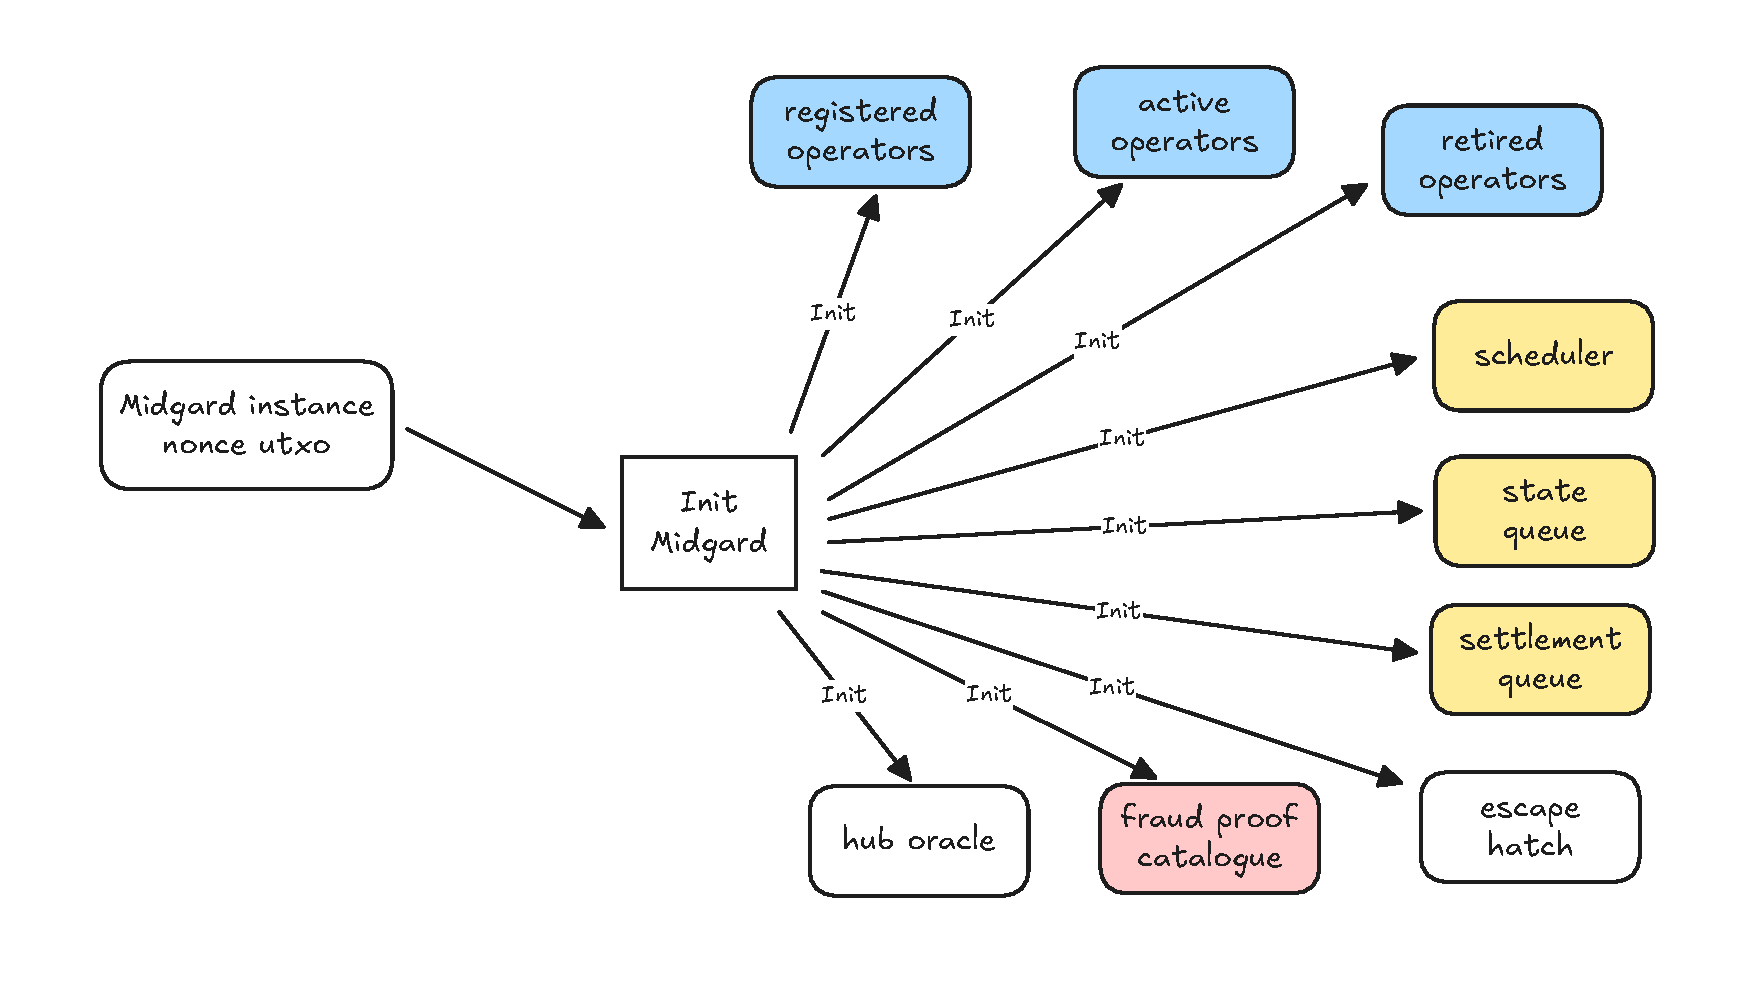
\includegraphics[width=\txDiagramScale\linewidth]{\subfix{../images/tx-diagram/0-init-midgard.pdf}}
\end{center}
\caption[Initialize Midgard]{Initialize Midgard.}
\label{fig:tx-init-midgard}
\end{figure}

Initialize a Midgard instance with a single transaction that sets up all the onchain data structures required for Midgard's smart-contract-based consensus protocol.
This transaction (\cref{fig:tx-init-midgard}):
\begin{enumerate}
  \item Spends a nonce utxo to uniquely parametrize%
    \footnote{A Midgard instance's hub oracle minting policy is parametrized on the nonce utxo spent in the initialization transaction, and all minting policies of the Midgard instance are parametrized on the hub oracle minting policy.}
    and authorize the initialization%
    \footnote{For example, if the nonce utxo is spent from a native script address, then initializing a Midgard instance parametrized by that nonce utxo must satisfy the signature and timing requirements of the native script.}
    of the Midgard instance.
  \item Produces the root nodes of the initially empty registered, active, and retired operator lists.
  \item Produces the root nodes of the initially empty state and settlement queues.
  \item Produces the scheduler, escape hatch, fraud proof catalogue, and hub oracle singleton utxos.
  \item Attaches the signatures necessary to spend the nonce utxo.
\end{enumerate}

Correctness is enforced by the hub oracle minting policy's Init redeemer (\cref{h:hub-oracle-minting-policy}).

\section{Operator management}%
\label{h:midgard-l1-tx-operator-management}%

Midgard has several transactions that manage operators by interacting with the data structures of the operator directory.

\begin{figure}[H]
\begin{center}
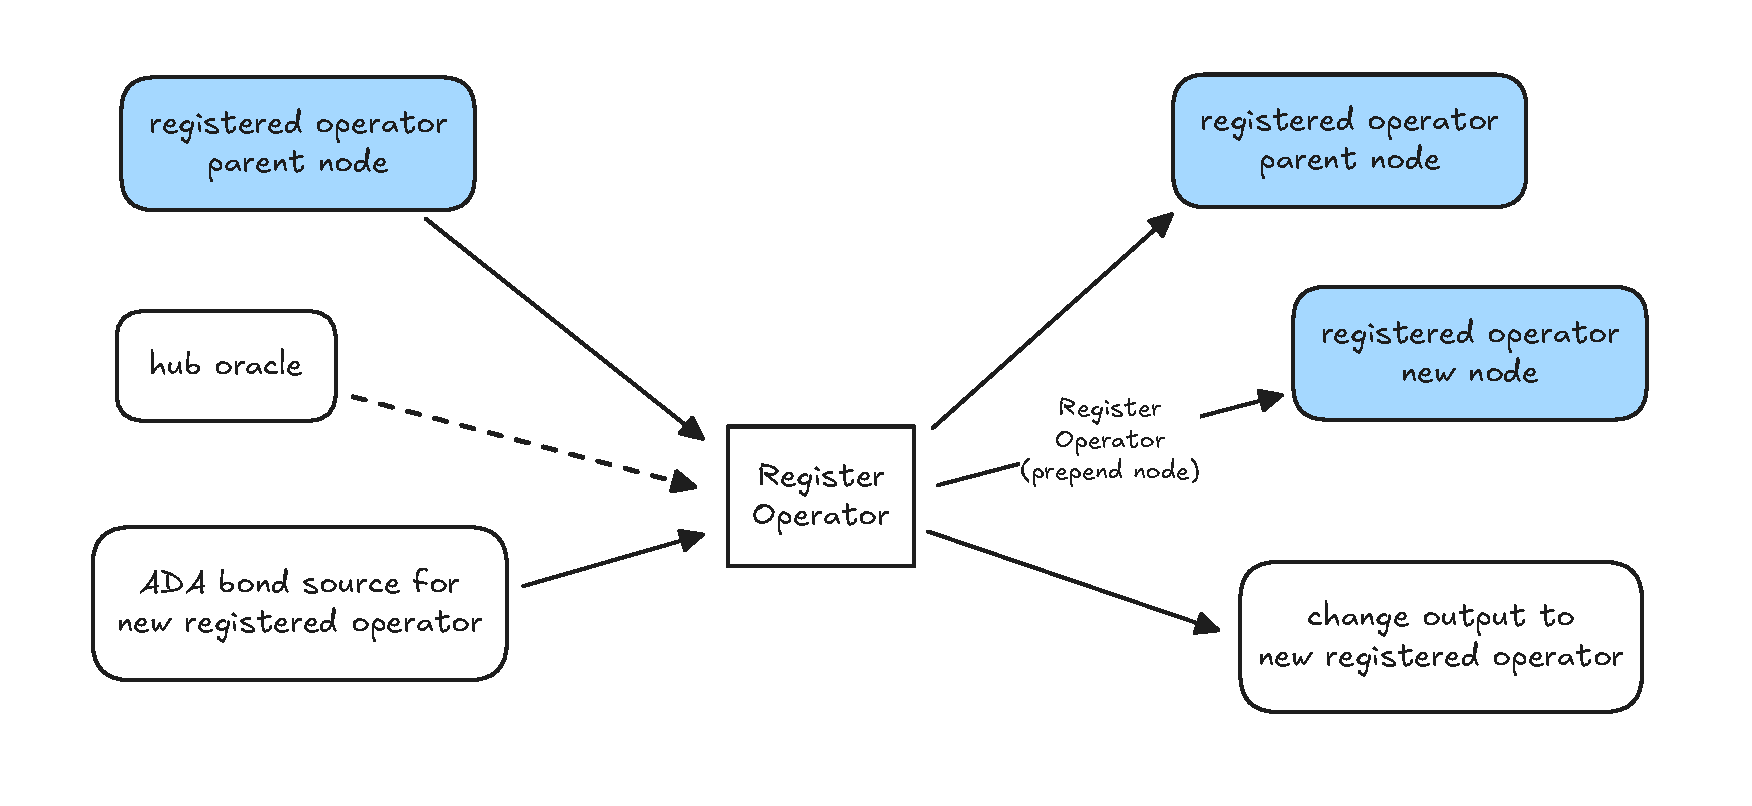
\includegraphics[width=\txDiagramScale\linewidth]{\subfix{../images/tx-diagram/1-register-operator.pdf}}
\end{center}
\caption[Register operator]{Register an operator.}
\label{fig:tx-register-operator}
\end{figure}

Register a new operator via a transaction that (\cref{fig:tx-register-operator}):
\begin{enumerate}
  \item Prepends a new operator node to the registered operators list. 
  \item Places a sufficient ADA bond into the new operator's node.
  \item Attaches the operator's signature to the transaction.
\end{enumerate}

Correctness is enforced by the registered operators minting policy's Register Operator redeemer (\cref{h:registered-operators-minting-policy}).

\begin{figure}[H]
\begin{center}
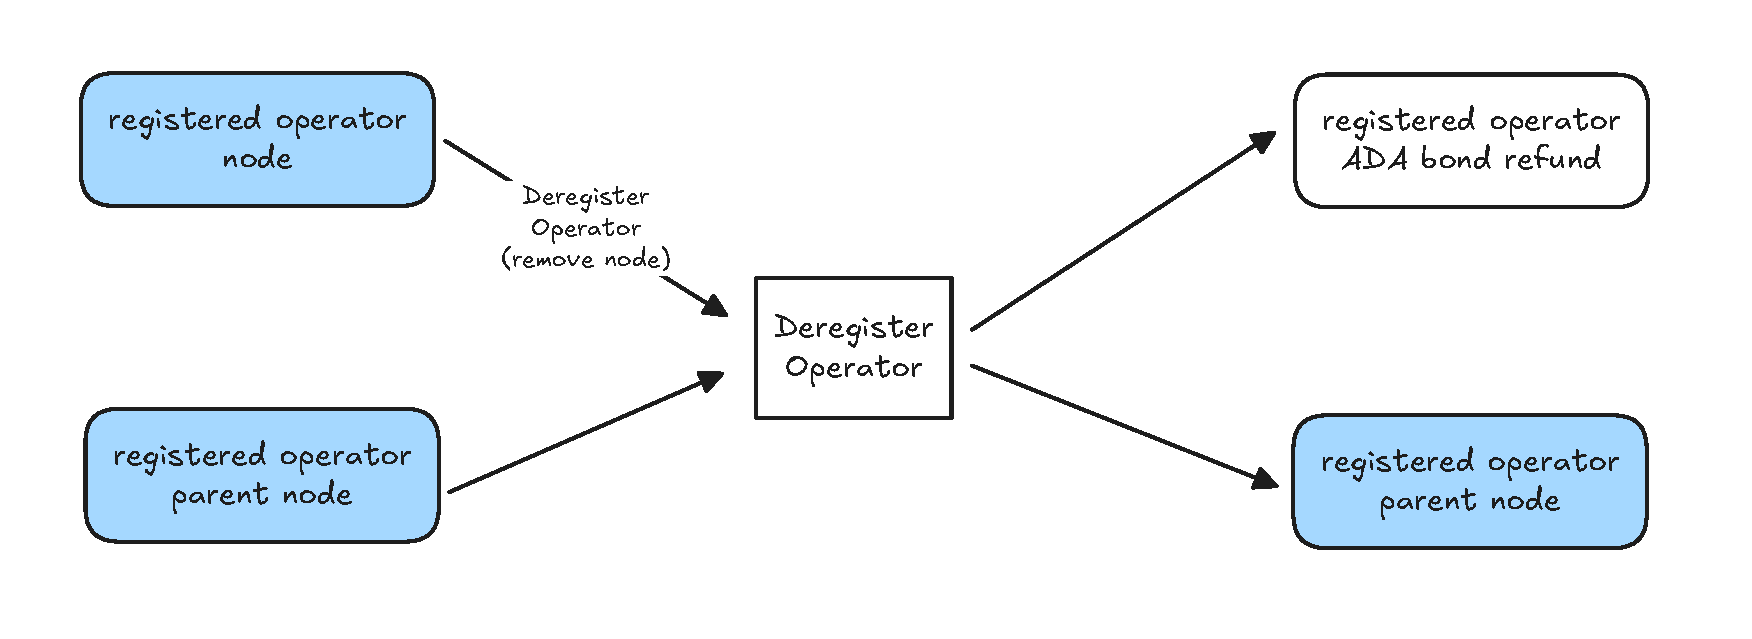
\includegraphics[width=\txDiagramScale\linewidth]{\subfix{../images/tx-diagram/2-deregister-operator.pdf}}
\end{center}
\caption[De-register operator]{De-register an operator.}
\label{fig:tx-deregister-operator}
\end{figure}

De-register an operator via a transaction that (\cref{fig:tx-deregister-operator}):
\begin{enumerate}
  \item Removes the operator's node from the registered operator's list.
  \item Refunds the ADA bond to the operator.
  \item Attaches the operator's signature to the transaction.
\end{enumerate}

Correctness is enforced by the registered operators minting policy's Deregister Operator redeemer (\cref{h:registered-operators-minting-policy}).

\begin{figure}[H]
\begin{center}
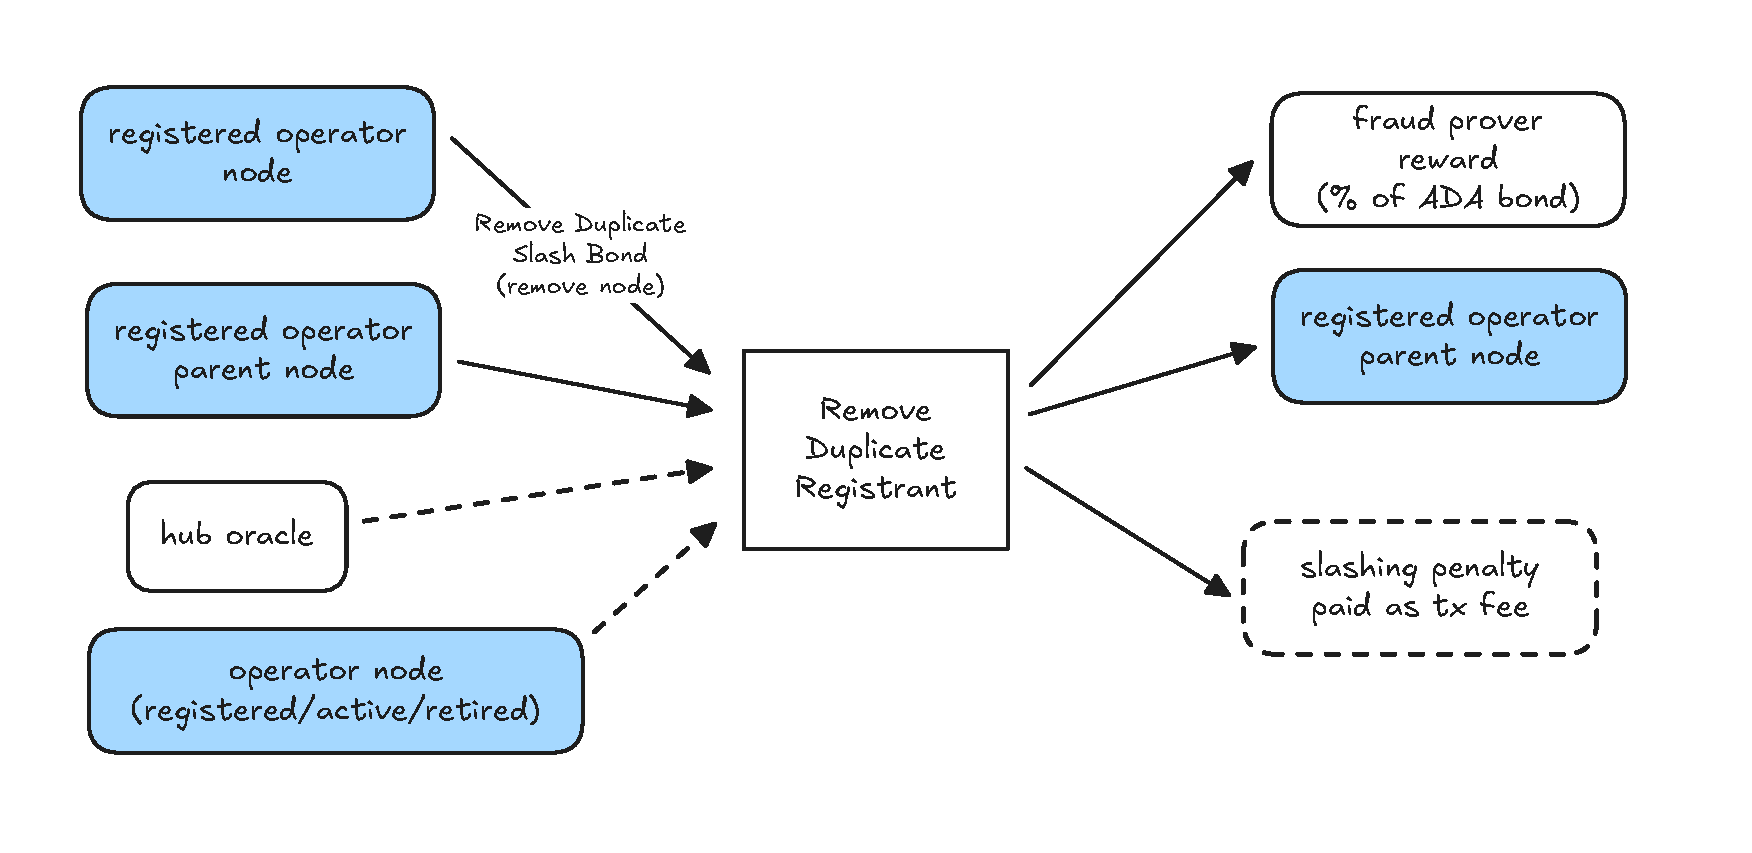
\includegraphics[width=\txDiagramScale\linewidth]{\subfix{../images/tx-diagram/3-remove-duplicate-registrant.pdf}}
\end{center}
\caption[Remove duplicate registrant]{Remove and slash a duplicate registered operator.}
\label{fig:tx-remove-duplicate-registrant}
\end{figure}

If the same operator key is simultaneously present in a registered operators node and in another node of the registered, active, or retired operators lists, then it can be removed via a transaction that (\cref{fig:tx-remove-duplicate-registrant}):
\begin{enumerate}
  \item Removes the duplicate node from the registered operators list
  \item Slashes the duplicate node's operator ADA bond, allocating part of it (\code{slashing\_penalty} param) to the transaction's fee and allowing the transaction submitter to claim the rest as the fraud prover reward.
  \item References the same operator key being used in another list node (registered/active/retired) to justify removing and slashing that operator's duplicate node.
\end{enumerate}

Correctness is enforced by the registered operators minting policy's Remove Duplicate Slash Bond redeemer (\cref{h:registered-operators-minting-policy}).

\begin{figure}[H]
\begin{center}
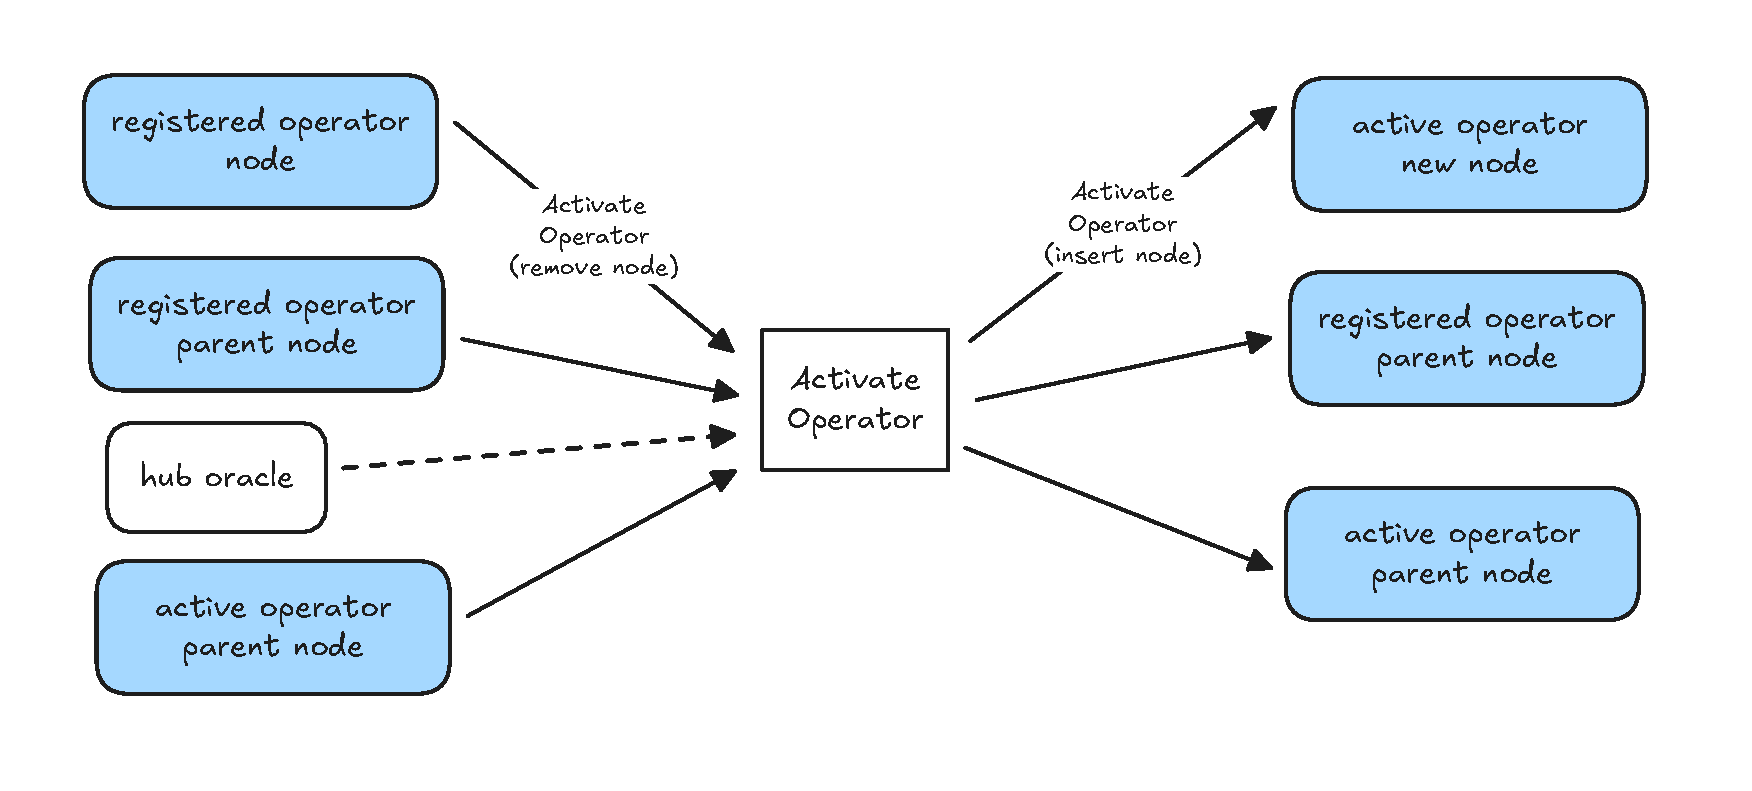
\includegraphics[width=\txDiagramScale\linewidth]{\subfix{../images/tx-diagram/4-activate-operator.pdf}}
\end{center}
\caption[Activate operator]{Activate a registered operator.}
\label{fig:tx-activate-operator}
\end{figure}

Activate an operator via a transaction that (\cref{fig:tx-activate-operator}):
\begin{enumerate}
  \item Removes the operator's node from the registered operators list.
  \item Inserts a node for the operator in the active operators list.
  \item Transfers the operator's ADA bond from the removed registered operator node to the inserted active operators node.
\end{enumerate}

Correctness is jointly enforced by these script redeemers:
\begin{itemize}
  \item Activate Operator of the registered operators minting policy (\cref{h:registered-operators-minting-policy}).
  \item Activate Operator of the active operators minting policy (\cref{h:active-operators-minting-policy}).
\end{itemize}

\begin{figure}[H]
\begin{center}
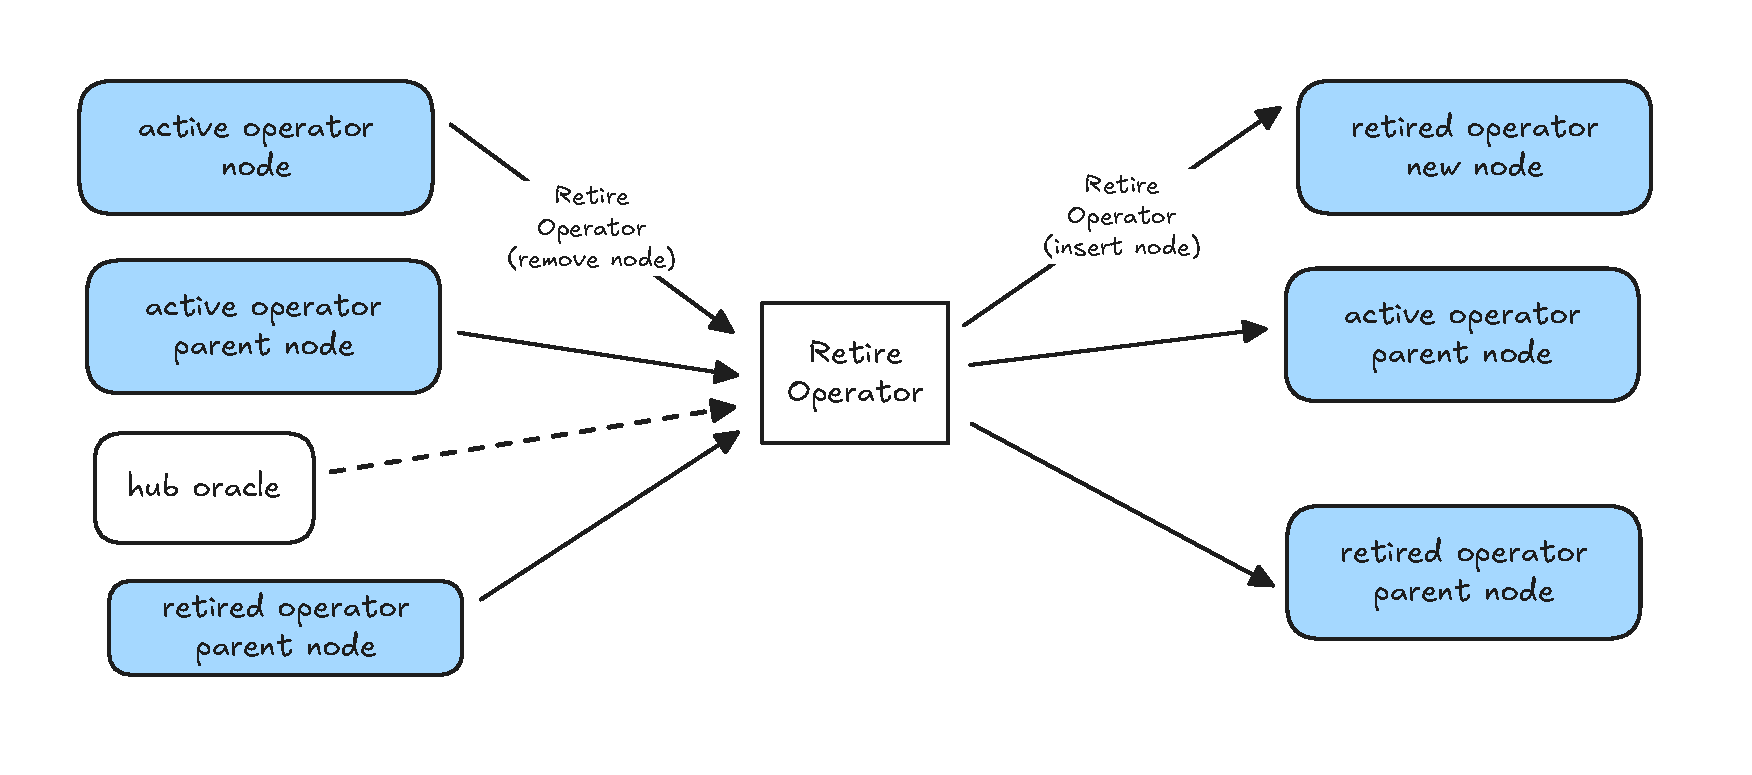
\includegraphics[width=\txDiagramScale\linewidth]{\subfix{../images/tx-diagram/5-retire-operator.pdf}}
\end{center}
\caption[Retire operator]{Retire an active operator.}
\label{fig:tx-retire-operator}
\end{figure}

Retire an operator via a transaction that (\cref{fig:tx-retire-operator}):
\begin{enumerate}
  \item Removes the operator's node from the active operators list.
  \item Inserts a node for the operator in the retired operators list.
  \item Transfers the operator's ADA bond from the removed active operator node to the inserted retired operator node.
  \item Attaches the operator's signature to the transaction.
\end{enumerate}

Correctness is jointly enforced by these script redeemers:
\begin{itemize}
  \item Retire Operator of the active operators minting policy (\cref{h:active-operators-minting-policy}).
  \item Retire Operator of the retired operators minting policy (\cref{h:retired-operators-minting-policy}).
\end{itemize}

\begin{figure}[H]
\begin{center}
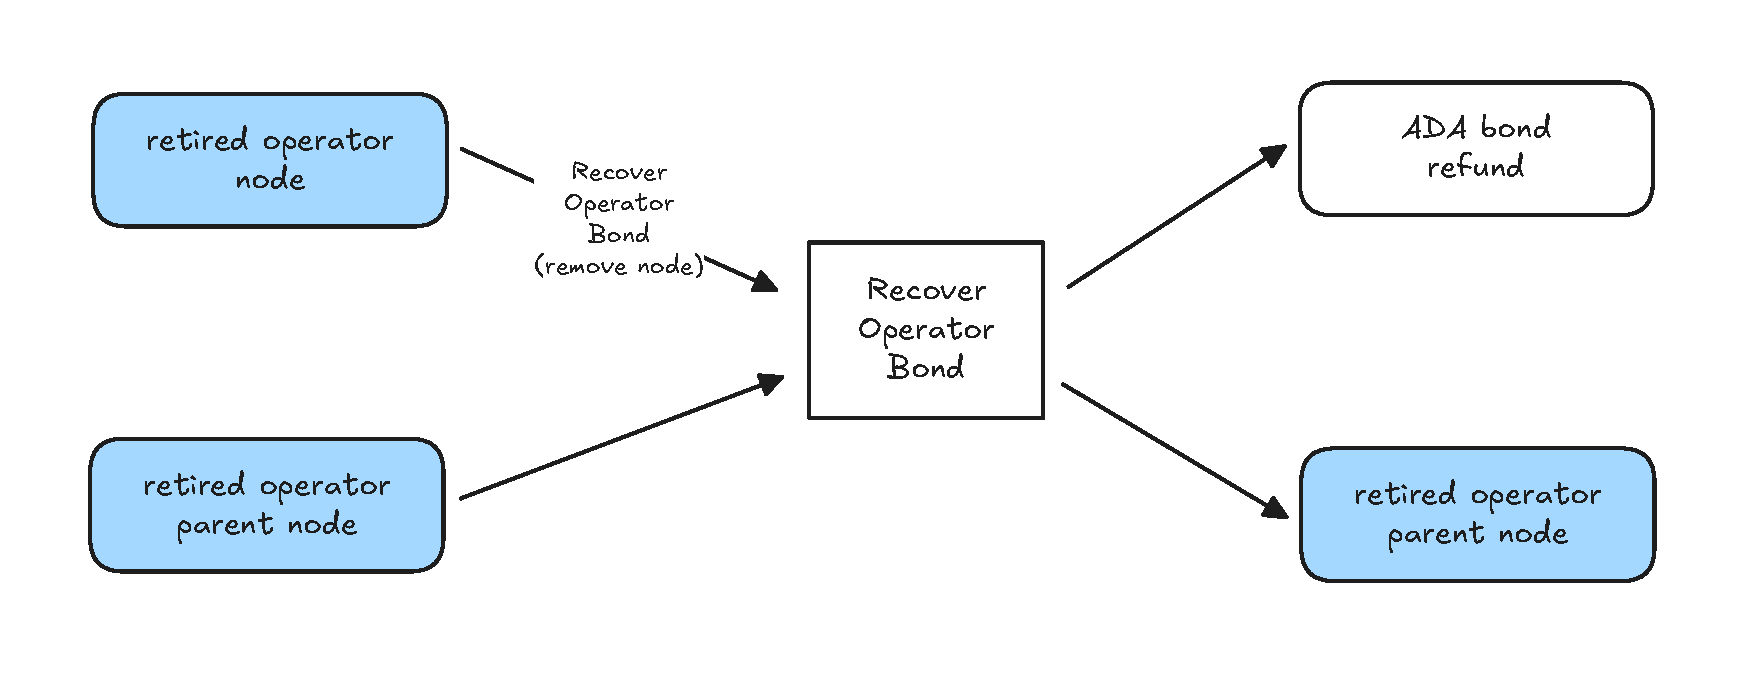
\includegraphics[width=\txDiagramScale\linewidth]{\subfix{../images/tx-diagram/6-recover-bond.pdf}}
\end{center}
\caption[Recover operator bond]{Recover a retired operator's bond.}
\label{fig:tx-recover-bond}
\end{figure}

After all of a retired operator's block headers (in the state queue) and resolution claims (in the settlement queue) have matured, the operator can recover his ADA bond via a transaction that (\cref{fig:tx-recover-bond}):
\begin{enumerate}
  \item Removes the operator's node from the retired operators list.
  \item Refunds the operator's ADA bond to the operator.
  \item Attaches the operator's signature to the transaction.
\end{enumerate}

Correctness is enforced by the retired operators minting policy's Recover Operator Bond redeemer (\cref{h:retired-operators-minting-policy}).

\section{Scheduler}%
\label{h:midgard-l1-tx-scheduler}%

\begin{figure}[H]
\begin{center}
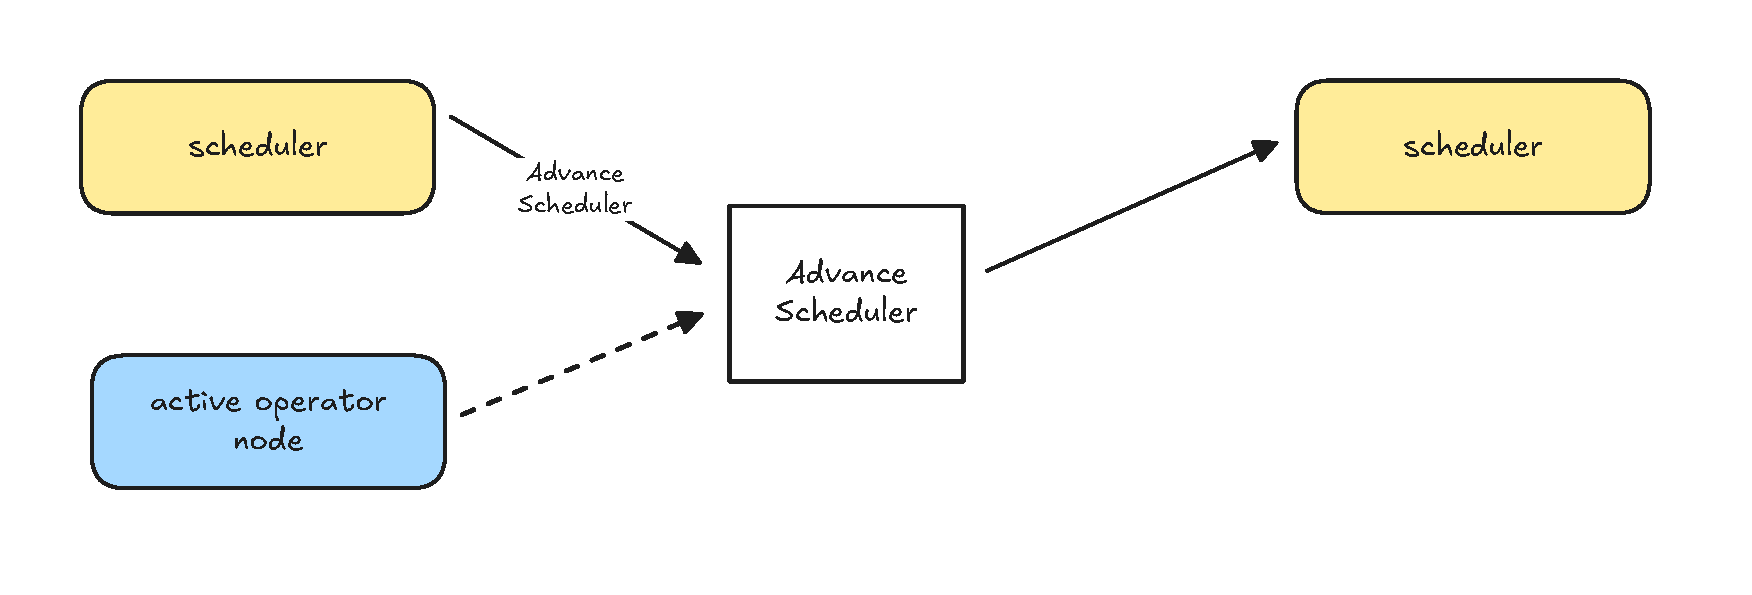
\includegraphics[width=\txDiagramScale\linewidth]{\subfix{../images/tx-diagram/7-advance-scheduler.pdf}}
\end{center}
\caption[Advance scheduler]{Advance the scheduler to the next operator.}
\label{fig:tx-advance-scheduler}
\end{figure}

Advance the scheduler via transaction that (\cref{fig:tx-advance-scheduler}):
\begin{enumerate}
  \item Updates the scheduler's datum to start the next shift and assign it to a new operator.
  \item References an active operator node that proves that the newly assigned operator follows the previously assigned operator in key-descending order of the active operators list.
\end{enumerate}

Correctness is enforced by the scheduler spending validator's Advance redeemer (\cref{h:scheduler-spending-validator}).

\begin{figure}[H]
\begin{center}
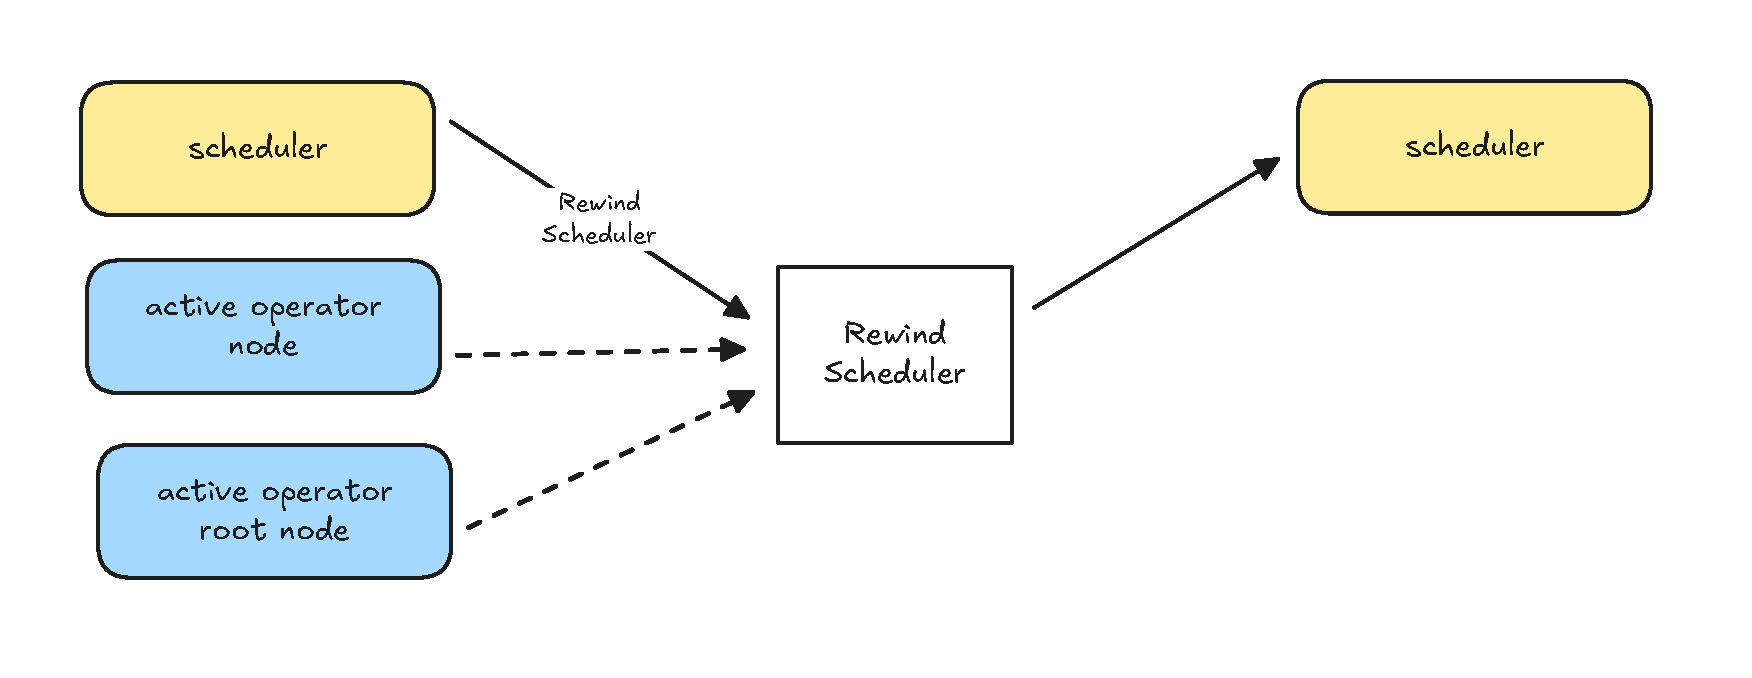
\includegraphics[width=\txDiagramScale\linewidth]{\subfix{../images/tx-diagram/8-rewind-scheduler.pdf}}
\end{center}
\caption[Rewind scheduler]{Rewind the scheduler to the first operator.}
\label{fig:tx-rewind-scheduler}
\end{figure}

Rewind the scheduler via a transaction that (\cref{fig:tx-rewind-scheduler}):
\begin{enumerate}
  \item Updates the scheduler's datum to the start the next shift and assign it to a new operator.
  \item References the active operators' root and last nodes to prove that the previously assigned operator was at the end and the newly assigned operator is at the beginning of the key-descending order of the active operators list.
\end{enumerate}

Correctness is enforced by the scheduler spending validator's Rewind redeemer (\cref{h:scheduler-spending-validator}).

\section{State queue}%
\label{h:midgard-l1-tx-state-queue}%

\begin{figure}[H]
\begin{center}
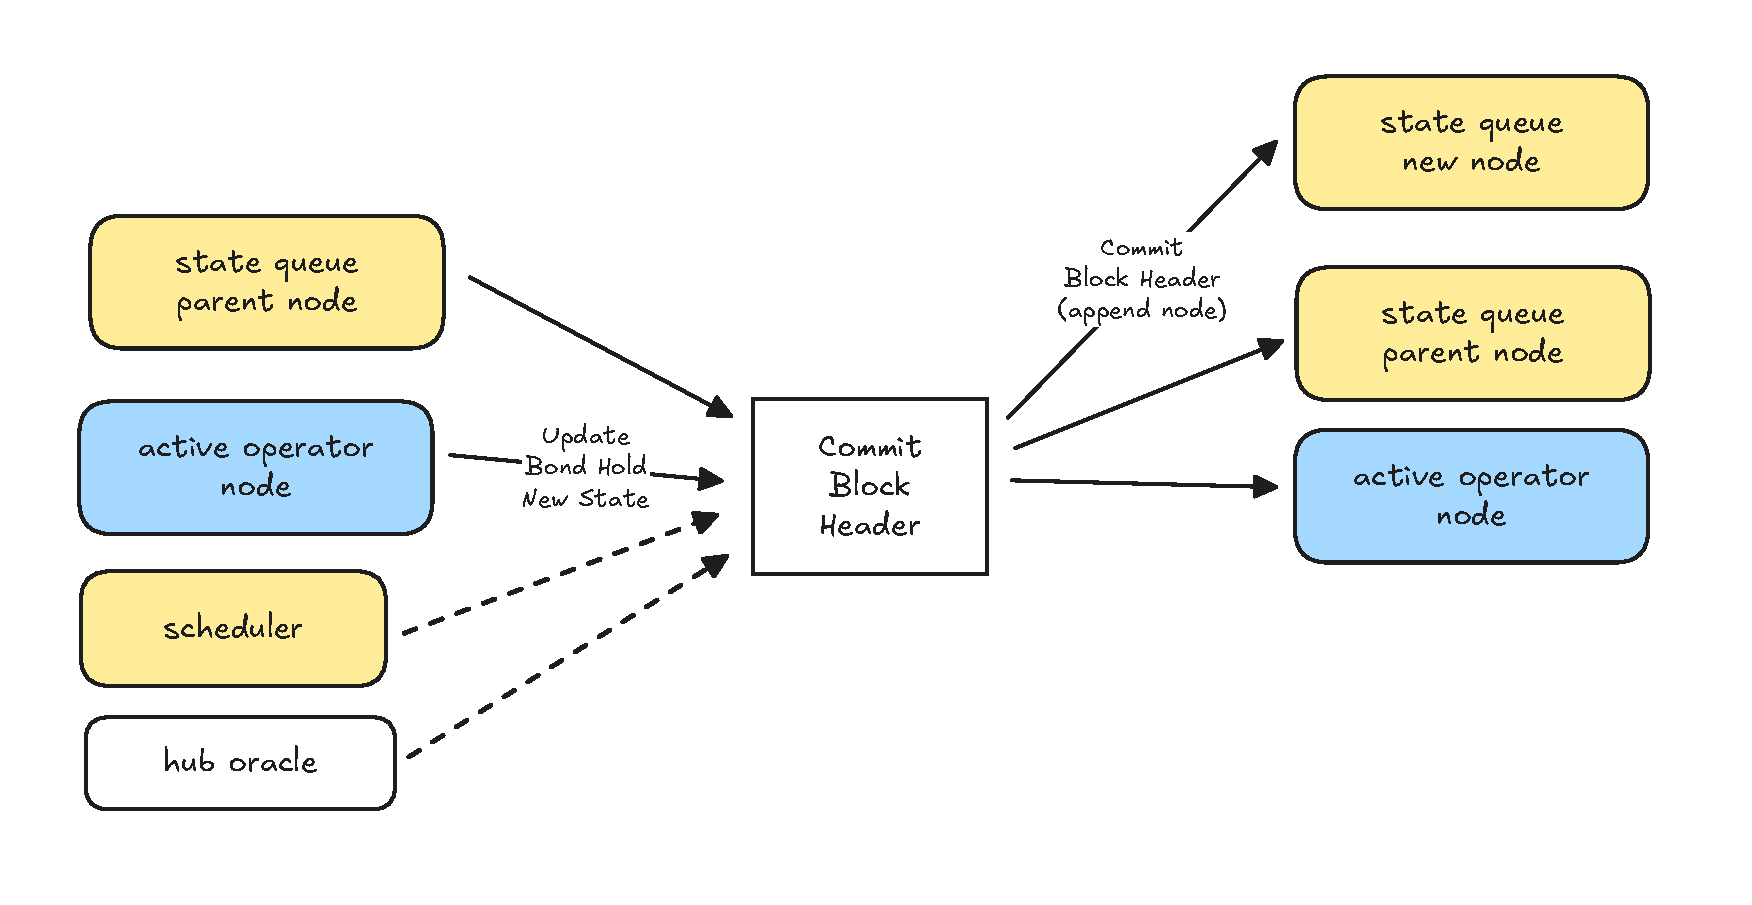
\includegraphics[width=\txDiagramScale\linewidth]{\subfix{../images/tx-diagram/9-commit-block-header.pdf}}
\end{center}
\caption[Commit block header]{Commit a block header to the state queue.}
\label{fig:tx-commit-block-header}
\end{figure}

Commit a new block header to the state queue via a transaction that (\cref{fig:tx-commit-block-header}):
\begin{enumerate}
  \item Appends a new node containing the block header to the state queue.
  \item Updates the operator's bond-unlock time to the future time when the new block header will mature.
  \item Attaches the operator's signature to the transaction.
  \item References the scheduler to verify that the operator has the right to commit a block during the current shift.
\end{enumerate}

Correctness is jointly enforced by these script redeemers:
\begin{itemize}
  \item Commit Block Header of the state queue minting policy (\cref{h:state-queue-minting-policy}).
  \item Update Bond Hold New State of the active operators spending validator (\cref{h:active-operators-spending-validator}).
\end{itemize}

\begin{figure}[H]
\begin{center}
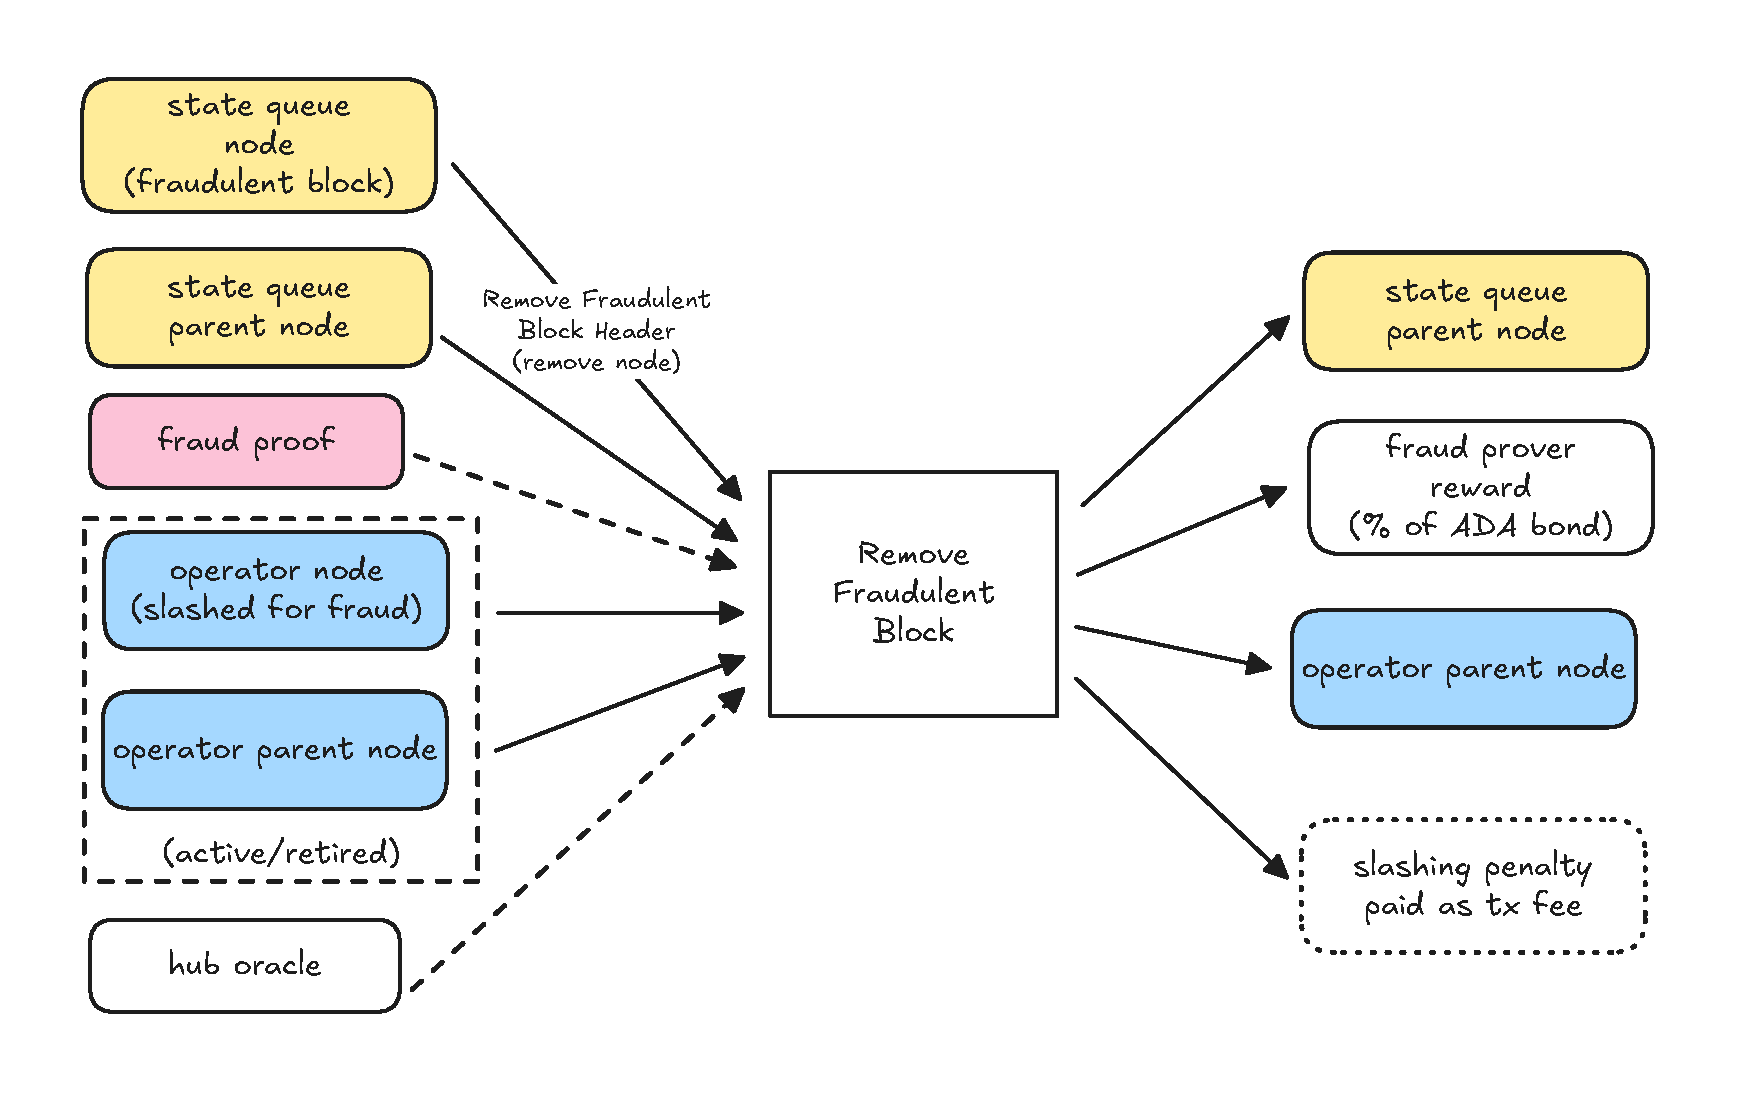
\includegraphics[width=\txDiagramScale\linewidth]{\subfix{../images/tx-diagram/A-remove-fraudulent-block-header.pdf}}
\end{center}
\caption[Remove fraudulent block header]{Remove a fraudulent block header and slash its operator.}
\label{fig:tx-remove-fraudulent-block-header}
\end{figure}

Remove a fraudulent block header from the state queue via a transaction that (\cref{fig:tx-remove-fraudulent-block-header}):
\begin{enumerate}
  \item References a fraud proof to justify removing the block header and slashing its operator.
  \item Removes the fraudulent block header's node from the state queue.
  \item Removes the dishonest operator's node from the active operators or retired operators list (depending on where the operator's node resides).
  \item Slashes the dishonest operator's ADA bond, sending part of it (\code{fraud\_prover\_reward} param) to the fraud prover and paying the rest (\code{slashing\_penalty}) as transaction fees.
\end{enumerate}

Correctness is jointly enforced by these script redeemers:
\begin{itemize}
  \item Remove Fraudulent Block Header of the state queue minting policy (\cref{h:state-queue-minting-policy}).
  \item Remove Operator Bad State of the active/retired operators minting policy (\cref{h:active-operators-minting-policy}, \cref{h:retired-operators-minting-policy}).
\end{itemize}

\begin{figure}[H]
\begin{center}
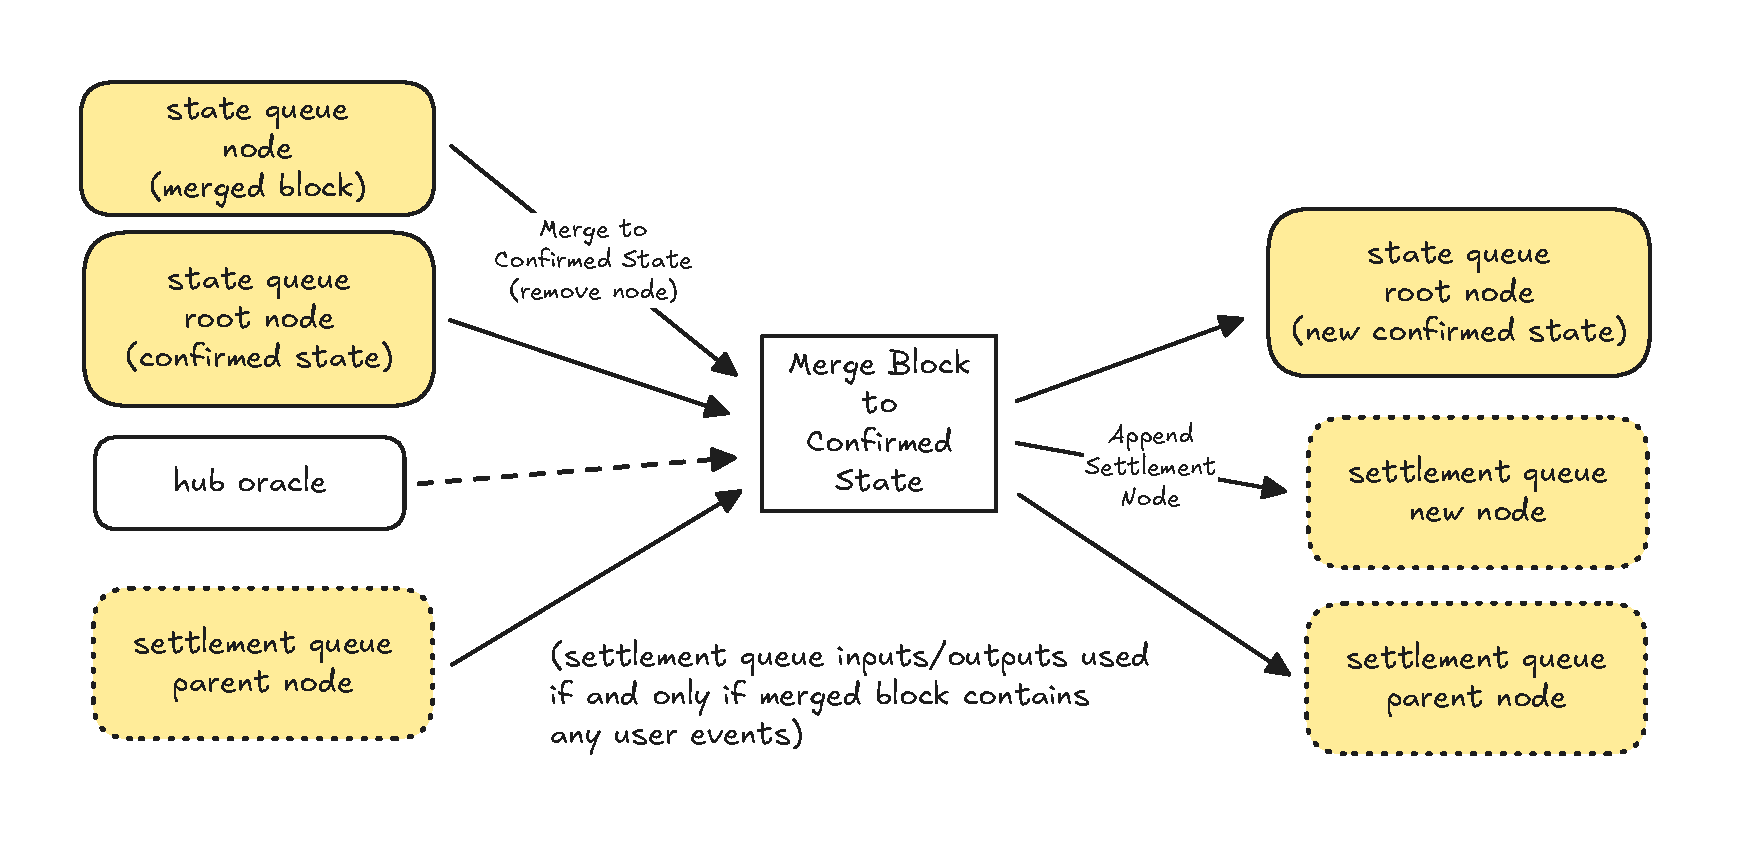
\includegraphics[width=\txDiagramScale\linewidth]{\subfix{../images/tx-diagram/B-merge-to-confirmed-state.pdf}}
\end{center}
\caption[Merge to confirmed state]{Merge a mature block header to the confirmed state.}
\label{fig:tx-merge-to-confirmed-state}
\end{figure}

Merge a matured block header to the confirmed state via a transaction that (\cref{fig:tx-merge-to-confirmed-state}):
\begin{enumerate}
  \item Removes the block header's node from the state queue.
  \item Updates the state queue's root node datum (i.e. Midgard's confirmed state) to the reflect the information contained in the block header.
  \item If the block header contains any L1 user events (deposits, transaction orders, or withdrawal orders) append a new node containing the same user events to the settlement queue.
\end{enumerate}

Correctness is jointly enforced by these script redeemers:
\begin{itemize}
  \item Merge to Confirmed State of the state queue minting policy (\cref{h:state-queue-minting-policy}).
  \item Append Settlement Node of the settlement queue minting policy (\cref{h:settlement-queue-minting-policy}).
\end{itemize}

\section{Settlement queue}%
\label{h:midgard-l1-tx-settlement-queue}%

\begin{figure}[H]
\begin{center}
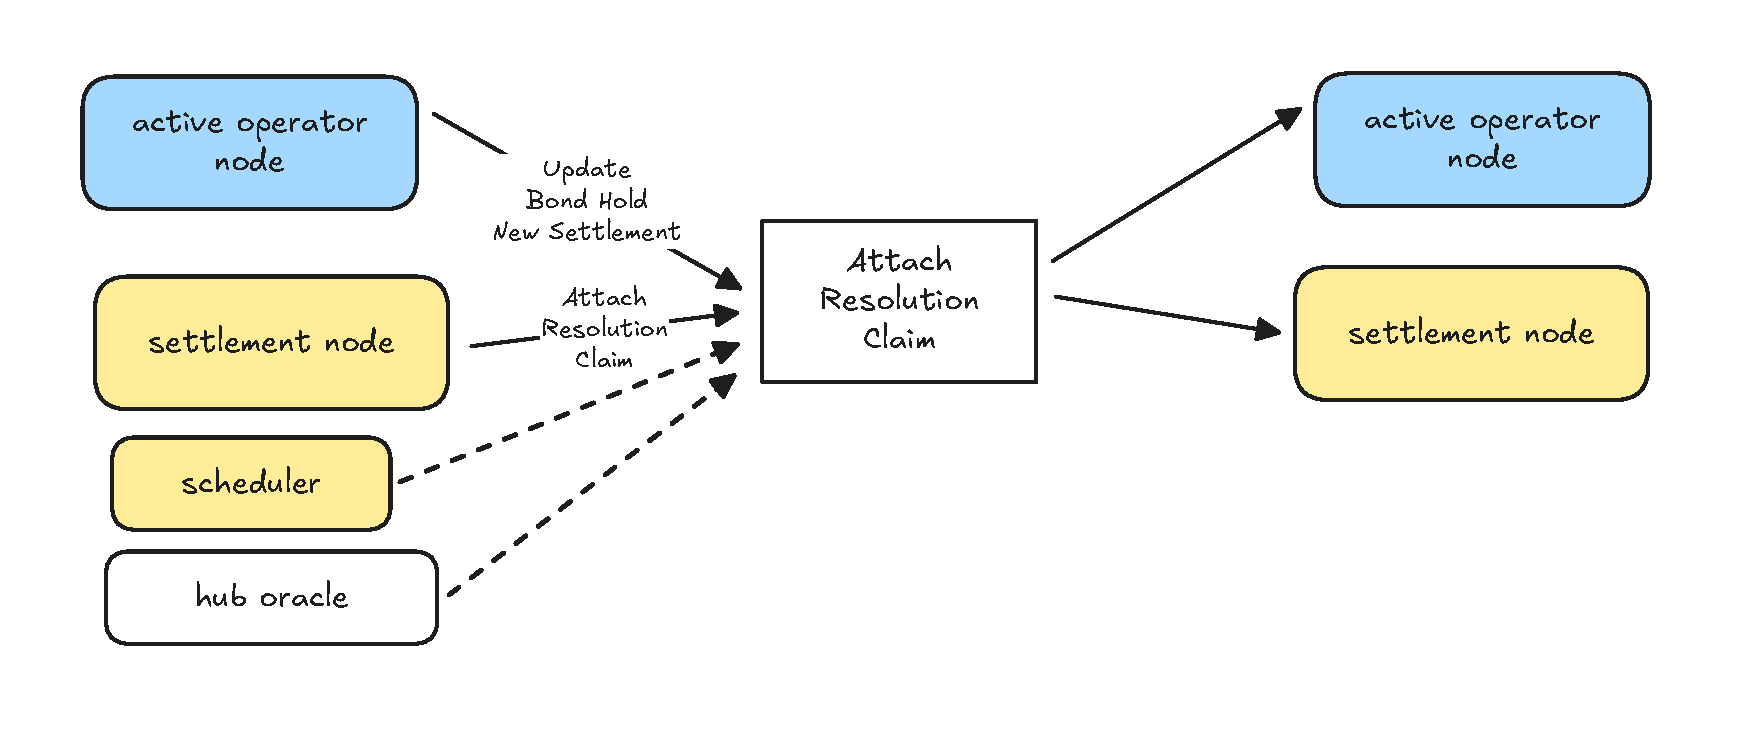
\includegraphics[width=\txDiagramScale\linewidth]{\subfix{../images/tx-diagram/C-attach-resolution-claim.pdf}}
\end{center}
\caption[Attach resolution claim]{Attach an optimistic resolution claim to a settlement node.}
\label{fig:tx-attach-resolution-claim}
\end{figure}

Attach a claim that all user events in a settlement node have been resolved, via a transaction that (\cref{fig:tx-attach-resolution-claim}):
\begin{enumerate}
  \item Spends a settlement node without a resolution claim and updates its datum to attach a resolution claim. The claim must indicate the operator attaching the claim and the future time when the claim will mature (must be set according to \code{maturity\_duration} param).
  \item Spends the operator's node (must be active) and updates its datum's bond unlock time to the resolution claim's maturity time.
  \item Attaches the operator's signature to the transaction.
  \item References the scheduler to demonstrate that the current shift is assigned to the operator attaching the resolution claim.
\end{enumerate}

Correctness is jointly enforced by these script redeemers:
\begin{itemize}
  \item Attach Resolution Claim of the settlement queue spending validator (\cref{h:settlement-queue-spending-validator}).
  \item Update Bond Hold New Settlement of the active operators spending validator (\cref{h:active-operators-spending-validator}).
\end{itemize}

\begin{figure}[H]
\begin{center}
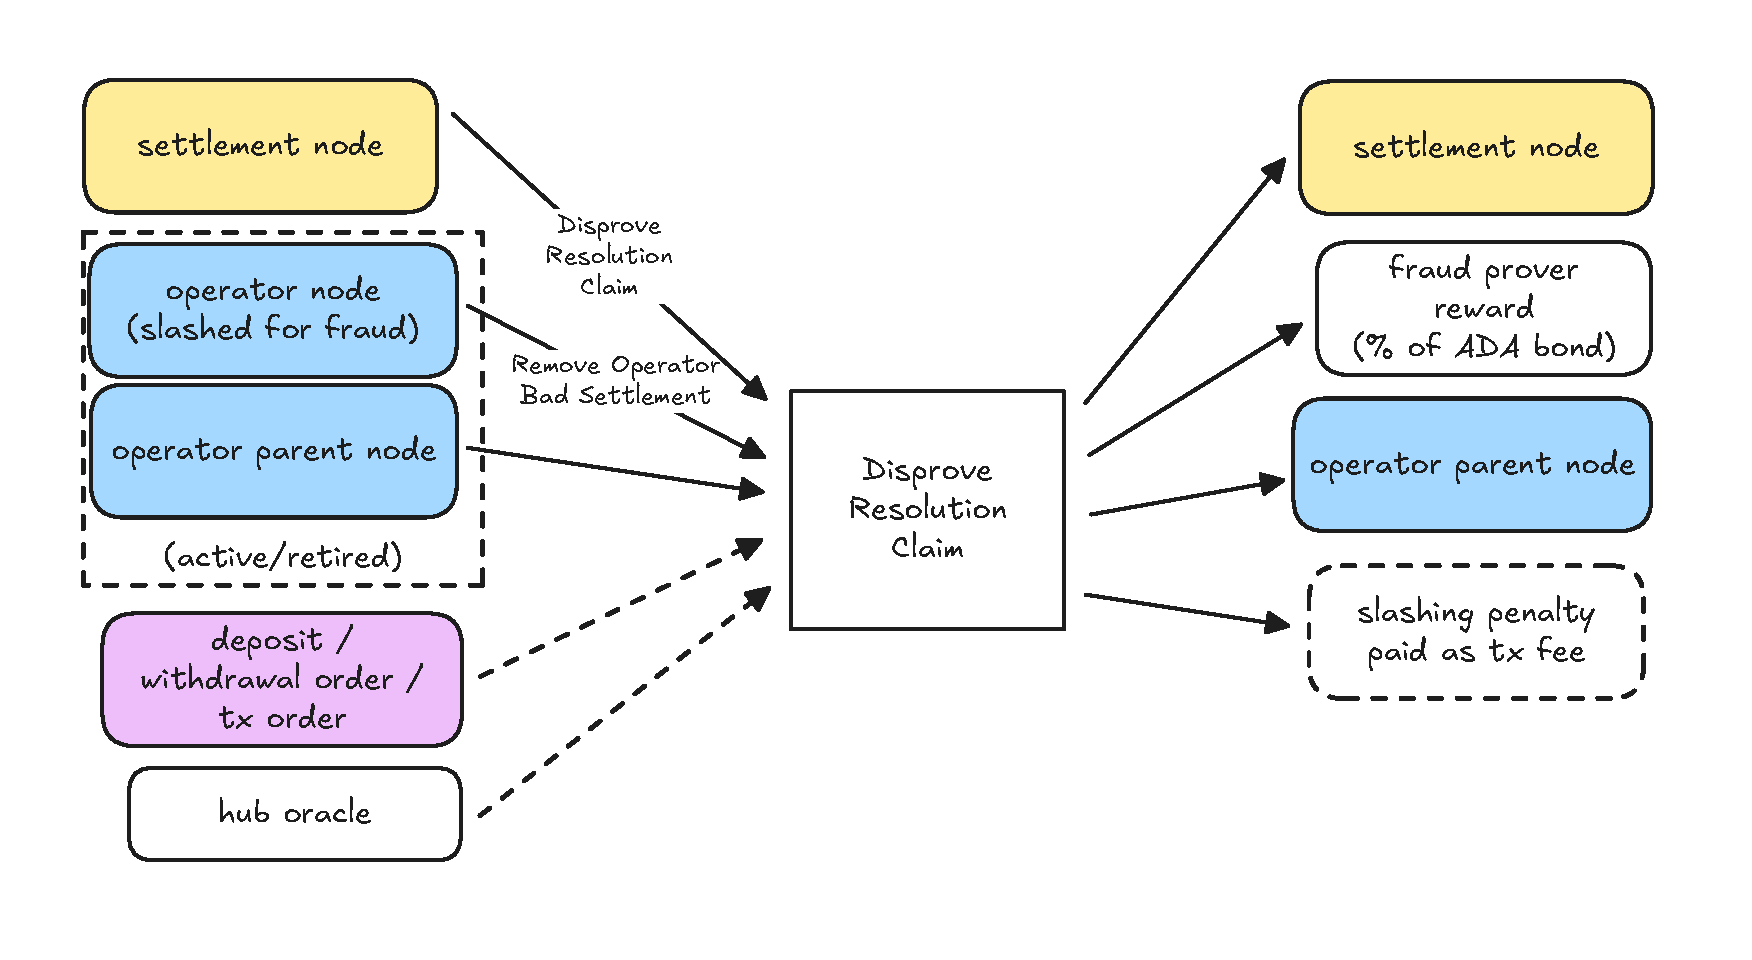
\includegraphics[width=\txDiagramScale\linewidth]{\subfix{../images/tx-diagram/D-disprove-resolution-claim.pdf}}
\end{center}
\caption[Disprove resolution claim]{Disprove an optimistic resolution claim of a settlement node.}
\label{fig:tx-disprove-resolution-claim}
\end{figure}

Disprove a settlement node's resolution claim via a transaction that (\cref{fig:tx-disprove-resolution-claim}):
\begin{enumerate}
  \item Spends a settlement node with a resolution claim and updates it to remove the resolution claim.
  \item Removes the resolution claim's operator node from the active operators or retired operators list (depending on where the operator's node resides).
  \item Slashes the dishonest operator's ADA bond, sending part of it (\code{fraud\_prover\_reward} param) to the transaction's submitter and paying the rest (\code{slashing\_penalty}) as transaction fees.
  \item References an L1 user event as a counter-example to the resolution claim---the event is included in the settlement node but has not yet been resolved.
\end{enumerate}

Correctness is jointly enforced by these script redeemers:
\begin{itemize}
  \item Disprove Resolution Claim of the settlement queue spending validator (\cref{h:settlement-queue-spending-validator}).
  \item Remove Operator Bad Settlement of the active operators or retired operators minting policy (\cref{h:active-operators-minting-policy}, \cref{h:retired-operators-minting-policy}).
\end{itemize}

\begin{figure}[H]
\begin{center}
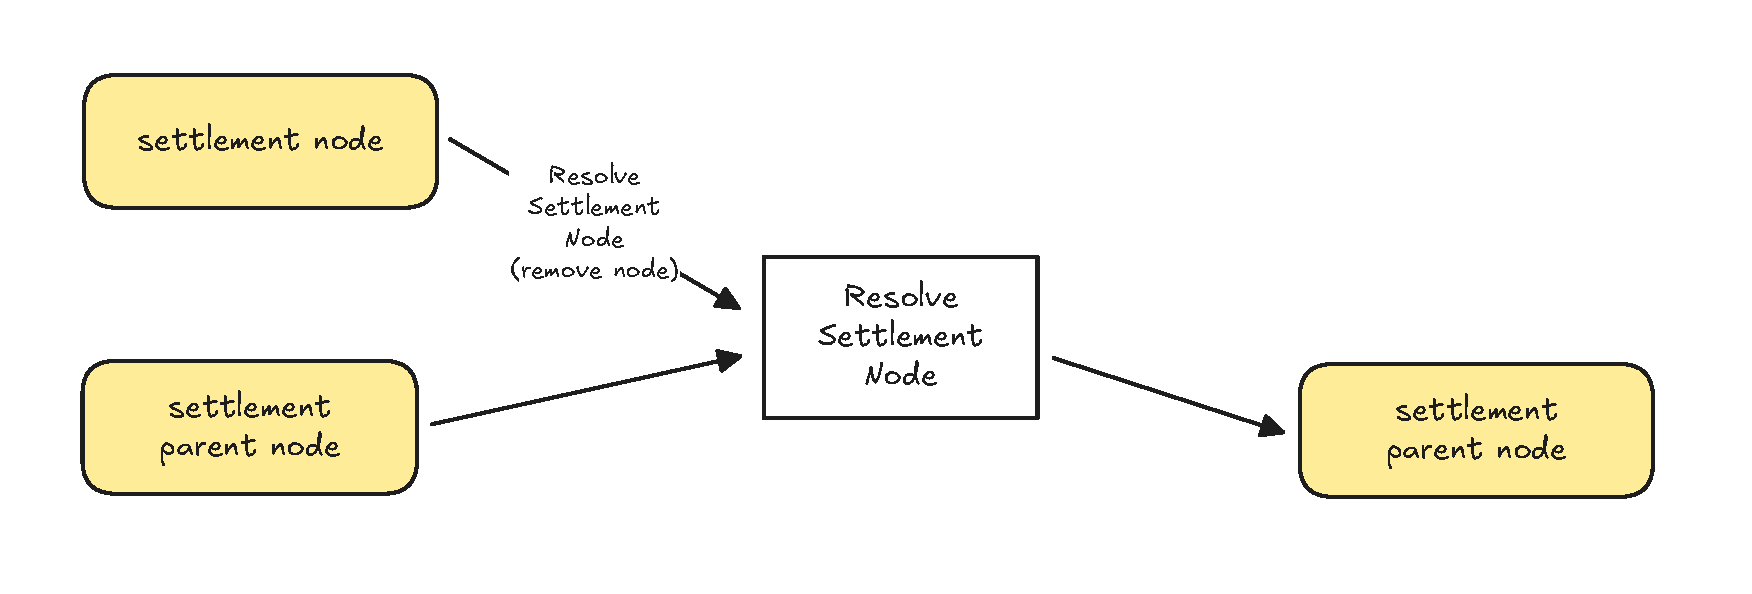
\includegraphics[width=\txDiagramScale\linewidth]{\subfix{../images/tx-diagram/E-resolve-settlement-node.pdf}}
\end{center}
\caption[Resolve settlement node]{Resolve a settlement node after its resolution claim matures.}
\label{fig:tx-resolve-settlement-node}
\end{figure}

Resolve a settlement node via a transaction that (\cref{fig:tx-resolve-settlement-node}):
\begin{enumerate}
  \item Removes a settlement queue node that contains a resolution claim with a maturity time preceding the transaction's time-validity lower bound.
  \item Attaches the signature of the resolution claim's operator.
\end{enumerate}

Correctness is enforced by the Resolve Settlement Node script redeemer of the settlement queue's minting policy (\cref{h:settlement-queue-minting-policy}).

\section{User events}%
\label{h:midgard-l1-tx-user-events}%

\begin{figure}[H]
\begin{center}
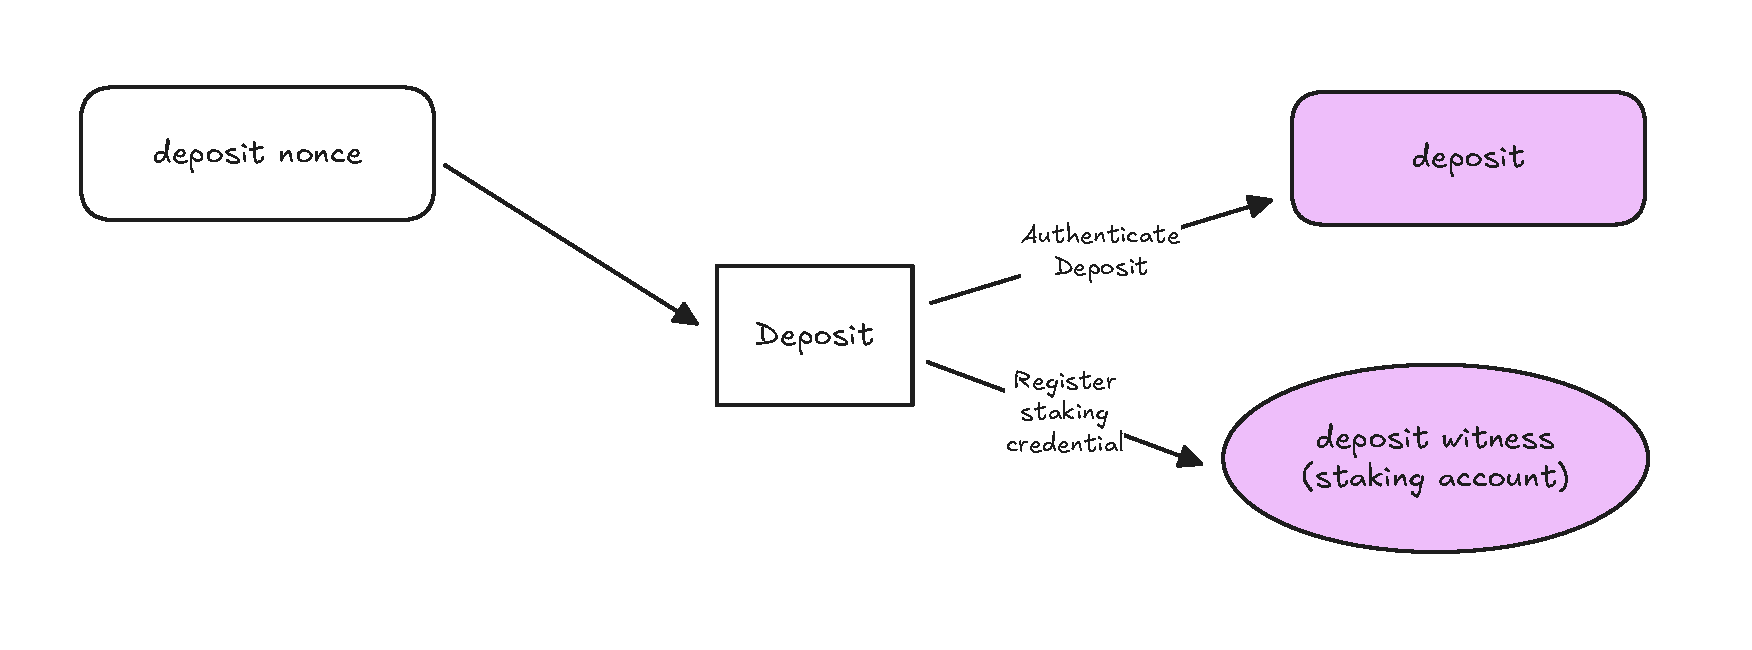
\includegraphics[width=\txDiagramScale\linewidth]{\subfix{../images/tx-diagram/F-deposit.pdf}}
\end{center}
\caption[Create deposit]{Create an L1 deposit for Midgard.}
\label{fig:tx-deposit}
\end{figure}

Create a new deposit for Midgard via a transaction that (\cref{fig:tx-deposit}):
\begin{enumerate}
  \item Spends a nonce input to uniquely parametrize the deposit.
  \item Produces a deposit utxo containing the user's deposited funds and instructions.
  \item Registers a staking credential to witness the existence of the deposit.
\end{enumerate}

Correctness is jointly enforced by these script redeemers:
\begin{itemize}
  \item Authenticate Deposit of the deposit minting policy (\cref{h:deposit-minting-policy}).
  \item Register Staking Credential of the witness staking script (\cref{h:witness-staking-script}).
\end{itemize}

\begin{figure}[H]
\begin{center}
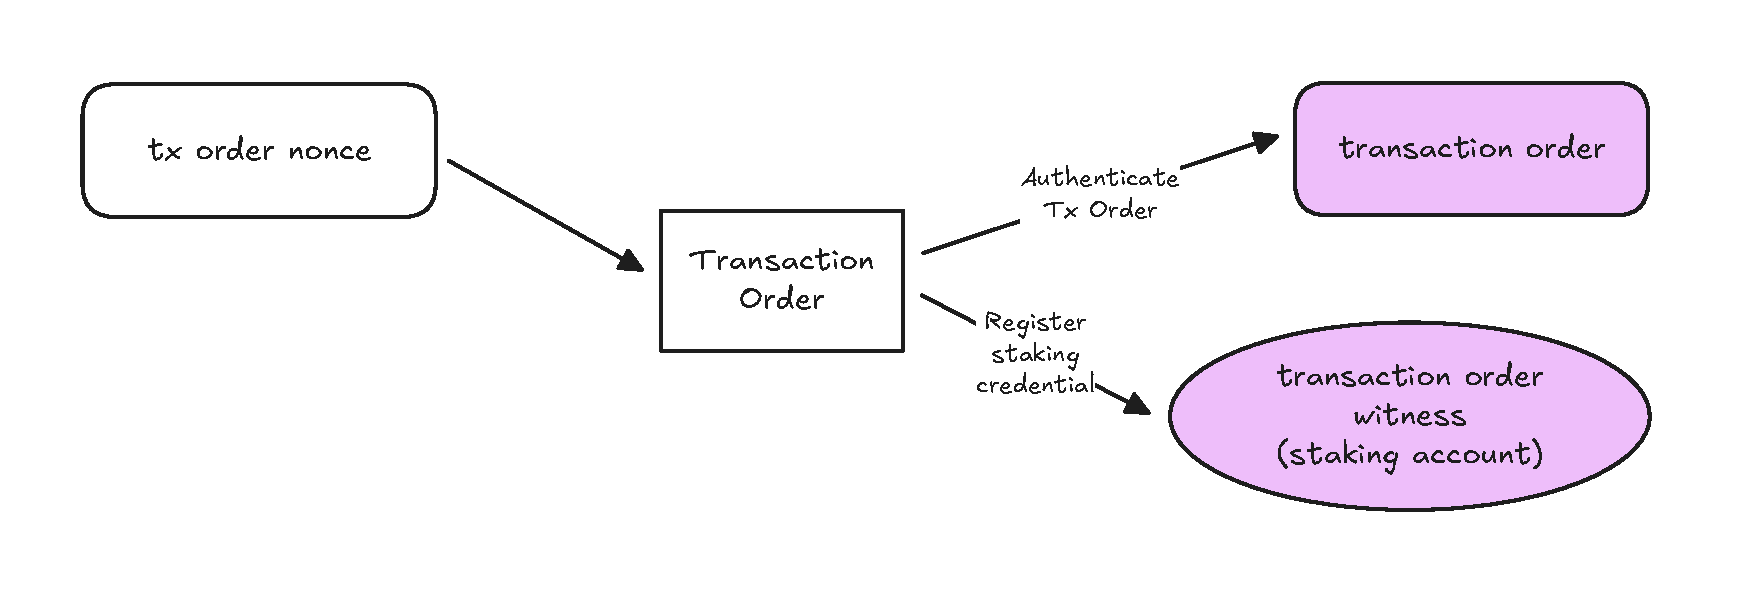
\includegraphics[width=\txDiagramScale\linewidth]{\subfix{../images/tx-diagram/G-tx-order.pdf}}
\end{center}
\caption[Create tx order]{Create a transaction order for Midgard.}
\label{fig:tx-transaction-order}
\end{figure}

Create a new transaction order for Midgard via a transaction that (\cref{fig:tx-transaction-order}):
\begin{enumerate}
  \item Spends a nonce input to uniquely parametrize the transaction order.
  \item Produces a transaction order utxo containing the user's L2 transaction.
  \item Registers a staking credential to witness the existence of the transaction order.
\end{enumerate}

Correctness is jointly enforced by these script redeemers:
\begin{itemize}
  \item Authenticate Transaction Order of the transaction order minting policy (\cref{h:transaction-order-minting-policy}).
  \item Register Staking Credential of the witness staking script (\cref{h:witness-staking-script}).
\end{itemize}

\begin{figure}[H]
\begin{center}
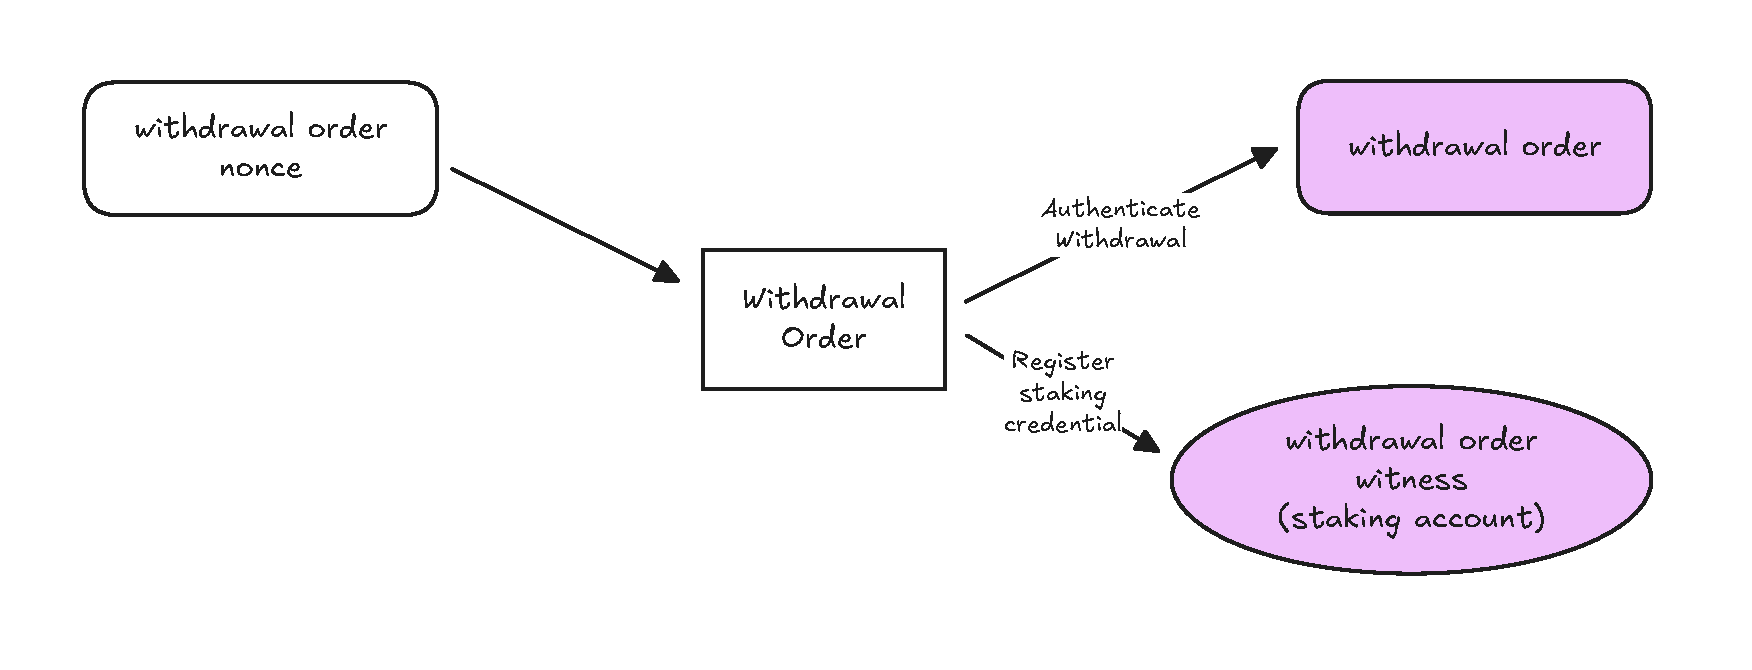
\includegraphics[width=\txDiagramScale\linewidth]{\subfix{../images/tx-diagram/H-withdrawal-order.pdf}}
\end{center}
\caption[Create withdrawal order]{Create a withdrawal order for Midgard.}
\label{fig:tx-withdrawal-order}
\end{figure}

Create a new withdrawal order for Midgard via a transaction that (\cref{fig:tx-transaction-order}):
\begin{enumerate}
  \item Spends a nonce input to uniquely parametrize the withdrawal order.
  \item Produces a withdrawal order utxo indicating the L2 utxo to be withdrawn.
  \item Registers a staking credential to witness the existence of the withdrawal order.
\end{enumerate}

Correctness is jointly enforced by these script redeemers:
\begin{itemize}
  \item Authenticate Withdrawal Order of the withdrawal order minting policy (\cref{h:transaction-order-minting-policy}).
  \item Register Staking Credential of the witness staking script (\cref{h:witness-staking-script}).
\end{itemize}

\begin{figure}[H]
\begin{center}
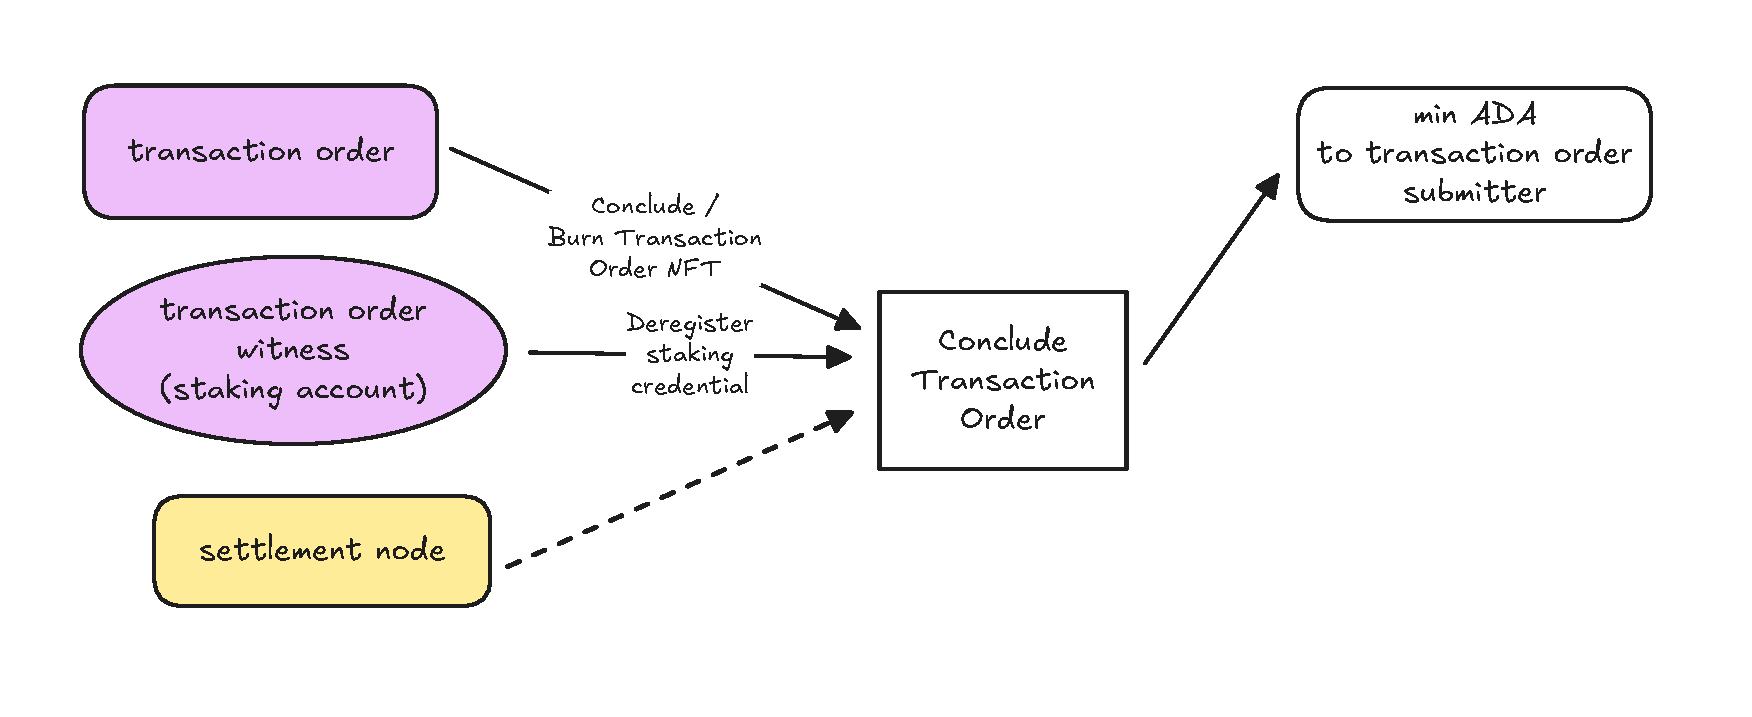
\includegraphics[width=\txDiagramScale\linewidth]{\subfix{../images/tx-diagram/I-conclude-tx-order.pdf}}
\end{center}
\caption[Conclude tx order]{Conclude a transaction order after it has been confirmed.}
\label{fig:tx-conclude-tx-order}
\end{figure}

Conclude a confirmed transaction order via a transaction that (\cref{fig:tx-conclude-tx-order}):
\begin{enumerate}
  \item Spends a transaction order and burns its NFT.
  \item De-registers the staking credential witnessing the transaction order.
  \item References a settlement node that includes the transaction order to prove that it has been confirmed.
\end{enumerate}

Correctness is jointly enforced by these script redeemers:
\begin{itemize}
  \item Conclude of the transaction order spending validator (\cref{h:transaction-order-spending-validator}).
  \item Burn Transaction Order NFT of the transaction order minting policy (\cref{h:transaction-order-minting-policy}).
  \item Mint or Burn of the witness staking script (\cref{h:witness-staking-script}).
\end{itemize}

\section{Reserve management}%
\label{h:midgard-l1-tx-reserve-management}%

\begin{figure}[H]
\begin{center}
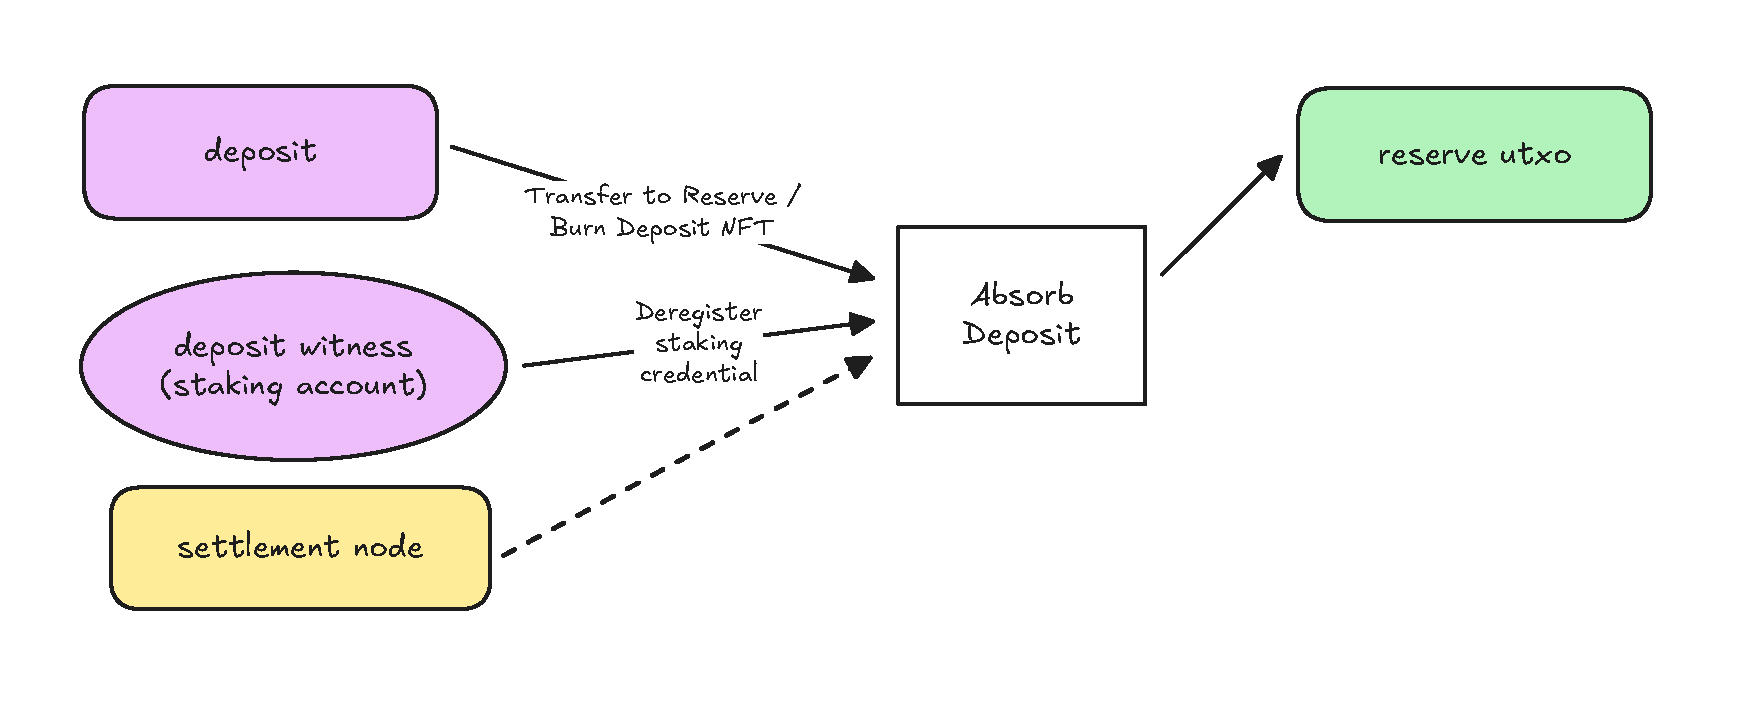
\includegraphics[width=\txDiagramScale\linewidth]{\subfix{../images/tx-diagram/J-absorb-deposit.pdf}}
\end{center}
\caption[Absorb deposit]{Absorb a deposit into the Midgard reserves after it has been confirmed.}
\label{fig:tx-absorb-deposit}
\end{figure}

Absorb a confirmed deposit into Midgard reserves via a transaction that (\cref{fig:tx-absorb-deposit}):
\begin{enumerate}
  \item Spends a deposit and burns its deposit NFT.
  \item De-registers the staking credential witnessing the deposit.
  \item References a settlement node that includes the deposit to prove that it has been confirmed.
\end{enumerate}

Correctness is jointly enforced by these script redeemers:
\begin{itemize}
  \item Transfer to Reserve of the deposit spending validator (\cref{h:deposit-spending-validator}).
  \item Burn Deposit NFt of the deposit minting policy (\cref{h:deposit-minting-policy}).
  \item Mint or Burn of the witness staking script (\cref{h:witness-staking-script}).
\end{itemize}

\begin{figure}[H]
\begin{center}
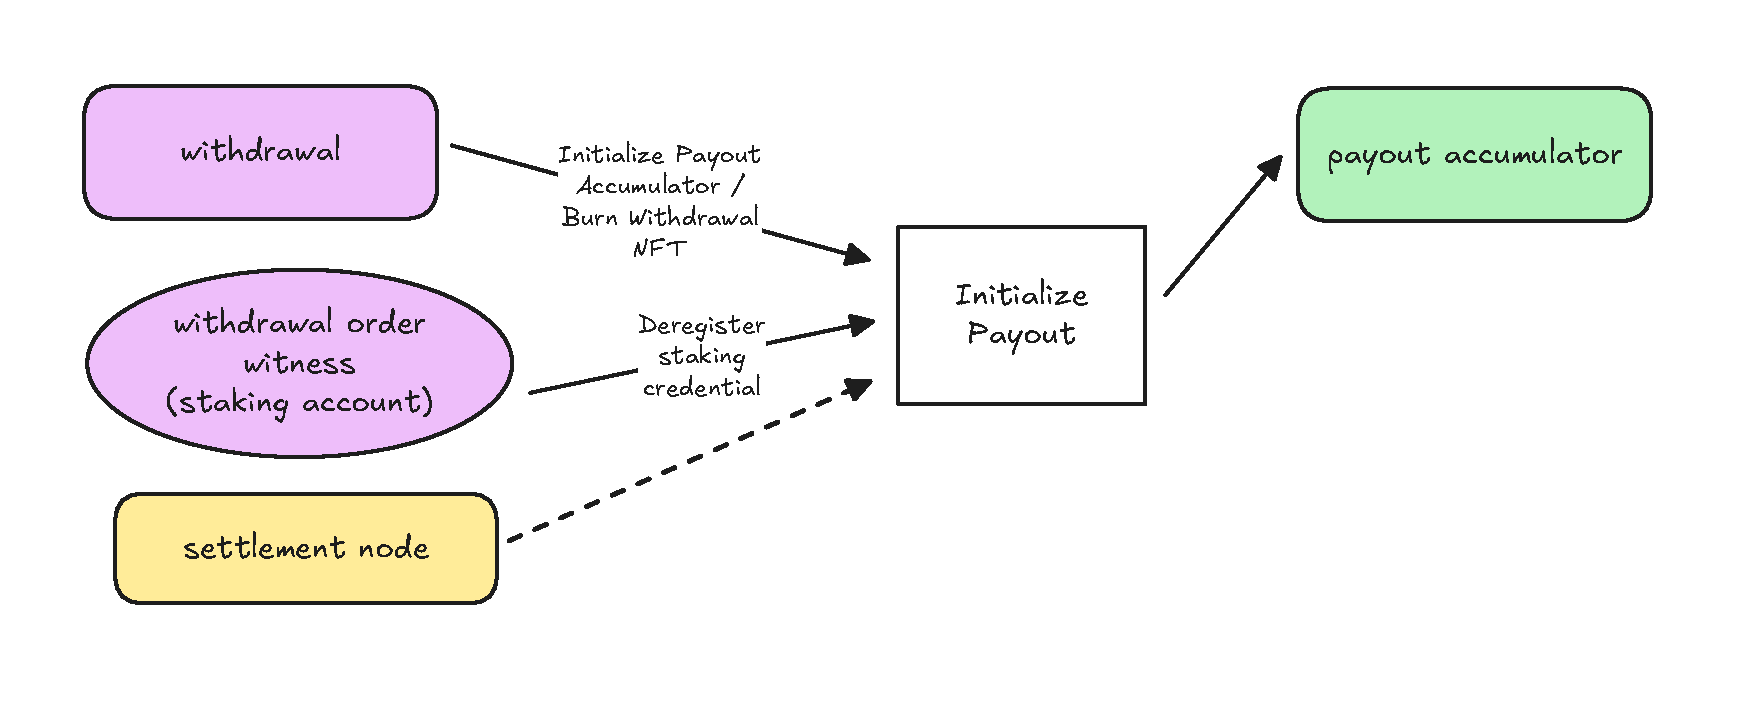
\includegraphics[width=\txDiagramScale\linewidth]{\subfix{../images/tx-diagram/K-init-payout-accumulator.pdf}}
\end{center}
\caption[Initialize payout accumulator]{Transform a confirmed withdrawal order into a payout accumulator.}
\label{fig:tx-initialize-payout-accumulator}
\end{figure}

Transform a confirmed withdrawal into a payout accumulator via a transaction that (\cref{fig:tx-initialize-payout-accumulator}):
\begin{enumerate}
  \item Spends the withdrawal order and burns its NFT.
  \item Produces a payout accumulator with \code{l2\_value}, \code{l1\_address}, and \code{l1\_datum} datum fields matching those of the withdrawal order.
  \item De-registers the staking credential witnessing the withdrawal order.
  \item References a settlement node that includes the withdrawal to prove that it has been confirmed.
\end{enumerate}

Correctness is jointly enforced by these script redeemers:
\begin{itemize}
  \item Initialize Payout Accumulator of the withdrawal order spending validator (\cref{h:withdrawal-order-spending-validator}).
  \item Burn Withdrawal NFT of the withdrawal order minting policy (\cref{h:withdrawal-order-minting-policy}).
  \item Burn or Mint of the witness staking script (\cref{h:witness-staking-script}).
\end{itemize}

\begin{figure}[H]
\begin{center}
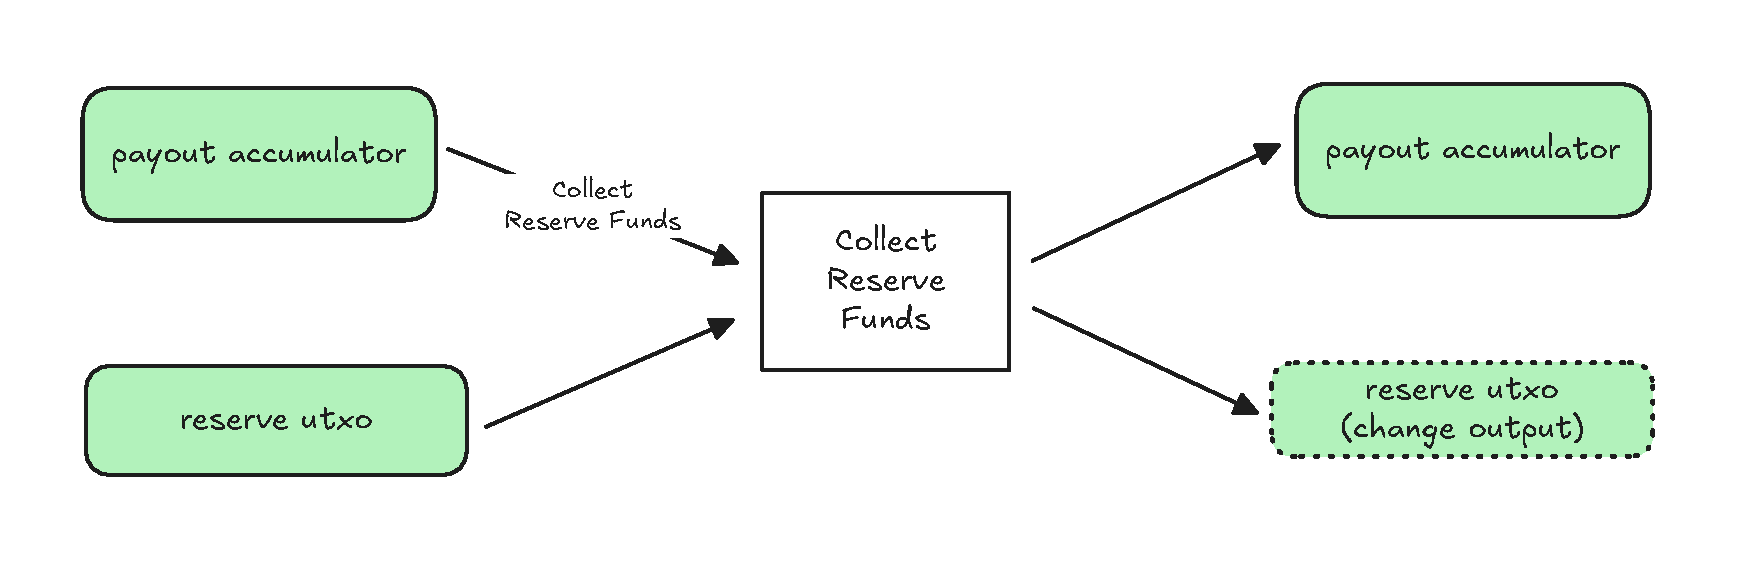
\includegraphics[width=\txDiagramScale\linewidth]{\subfix{../images/tx-diagram/L-collect-reserve-funds.pdf}}
\end{center}
\caption[Collect reserve funds]{Collect funds from Midgard reserves into a payout accumulator.}
\label{fig:tx-collect-reserve-funds}
\end{figure}

Collect funds from Midgard reserves into a payout accumulator via a transaction that (\cref{fig:tx-collect-reserve-funds}):
\begin{enumerate}
  \item Spends a payout accumulator.
  \item Spends a reserve utxo.
  \item Produces a payout accumulator output that combines the funds from the payout accumulator input with as many funds from the reserve utxo input as possible, up to the limit defined in the payout accumulator's \code{l2\_value} datum field.
  \item Produces a reserve utxo if needed to hold the remainder of the funds.
\end{enumerate}

Correctness is jointly enforced by these script redeemers:
\begin{itemize}
  \item Collect Reserve Funds of the payout accumulator spending validator (\cref{h:payout-accumulator-spending-validator})
  \item The sole redeemer of the reserve spending validator (\cref{h:reserve-spending-validator}).
\end{itemize}

\begin{figure}[H]
\begin{center}
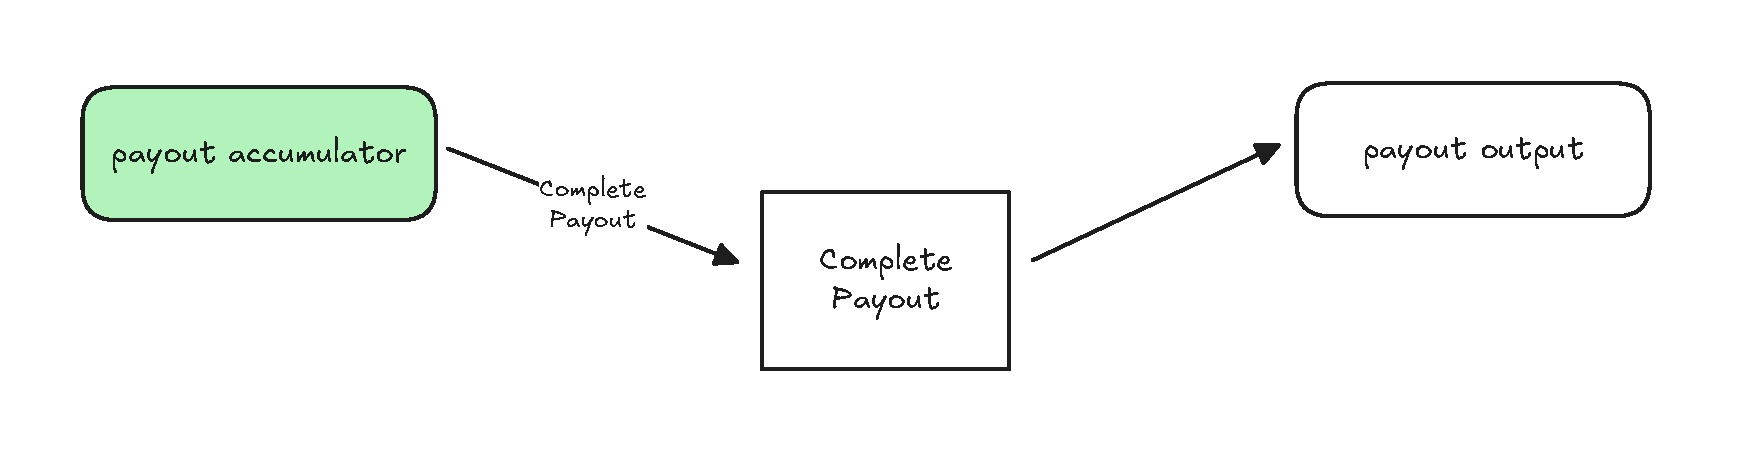
\includegraphics[width=\txDiagramScale\linewidth]{\subfix{../images/tx-diagram/M-complete-payout.pdf}}
\end{center}
\caption[Conclude payout]{Conclude a payout from Midgard.}
\label{fig:tx-conclude-payout}
\end{figure}

Conclude a payout from Midgard via a transaction that (\cref{fig:tx-conclude-payout}):
\begin{enumerate}
  \item Spends a payout accumulator with funds matching or exceeding the amount defined in its \code{l2\_value} datum field.
  \item Produces an output at the address and datum defined by the payout accumulator's \code{l1\_address} and \code{l1\_datum} datum fields.
\end{enumerate}

Correctness is jointly enforced by these script redeemers:
\begin{itemize}
  \item Complete Payout of the payout accumulator spending validator (\cref{h:payout-accumulator-spending-validator}).
  \item Burn of the payout accumulator minting policy (\cref{h:payout-accumulator-minting-policy}).
\end{itemize}

\section{Fraud proofs}%
\label{h:midgard-l1-tx-fraud-proofs}%

\begin{figure}[H]
\begin{center}
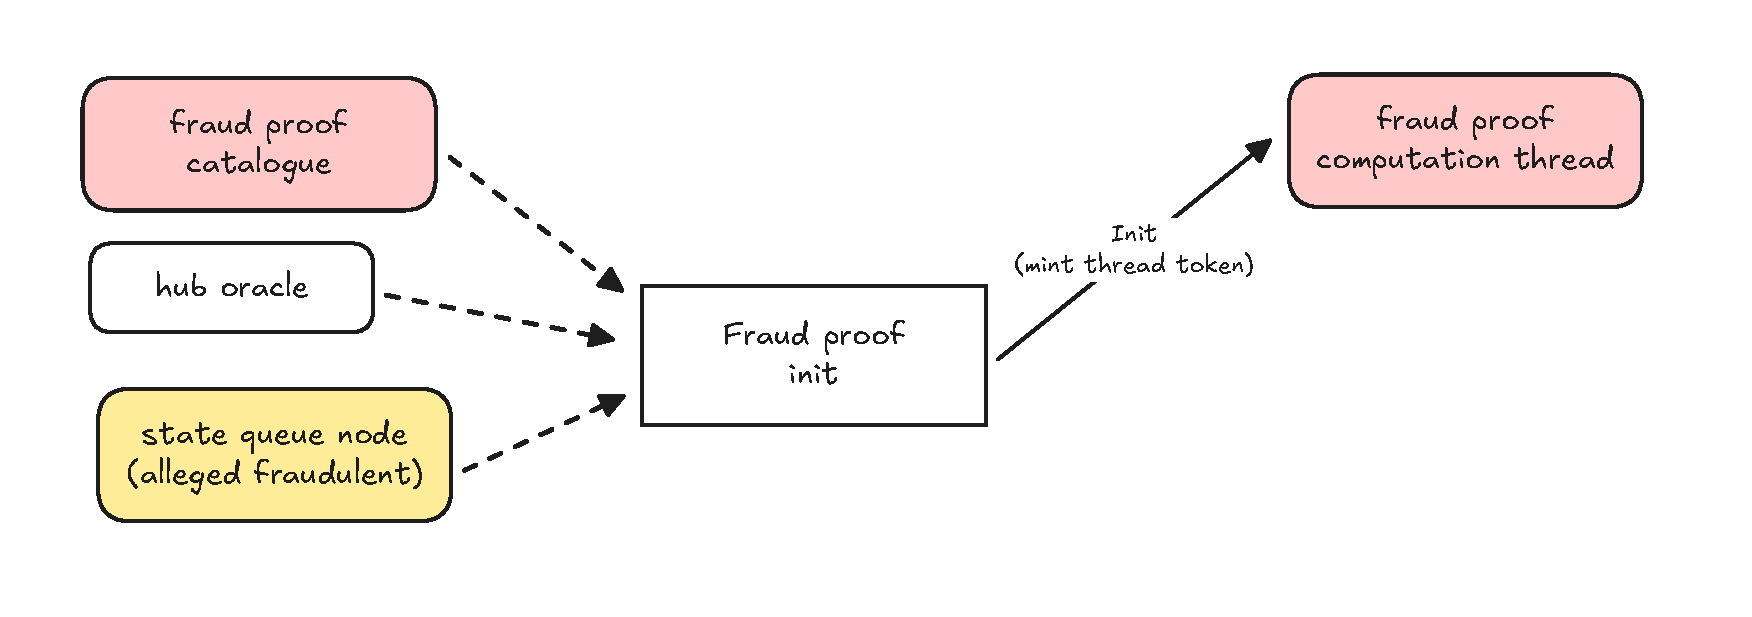
\includegraphics[width=\txDiagramScale\linewidth]{\subfix{../images/tx-diagram/N-fraud-proof-init.pdf}}
\end{center}
\caption[Fraud proof init]{Initialize the verification of a fraud proof.}
\label{fig:tx-fraud-proof-init}
\end{figure}

Initialize the verification of a fraud proof via a transaction that (\cref{fig:tx-fraud-proof-init}):
\begin{enumerate}
  \item References an allegedly fraudulent node in the state queue.
  \item References the fraud proof catalogue to select the fraud proof verification procedure that will demonstrate the allegation.
  \item Mints a computation thread token and sends it to the first step spending validator of the selected fraud proof verification procedure.
\end{enumerate}

Correctness is enforced by the Init redeemer of the fraud proof computation thread minting policy (\cref{h:fraud-proof-computation-threads-minting-policy}).

\begin{figure}[H]
\begin{center}
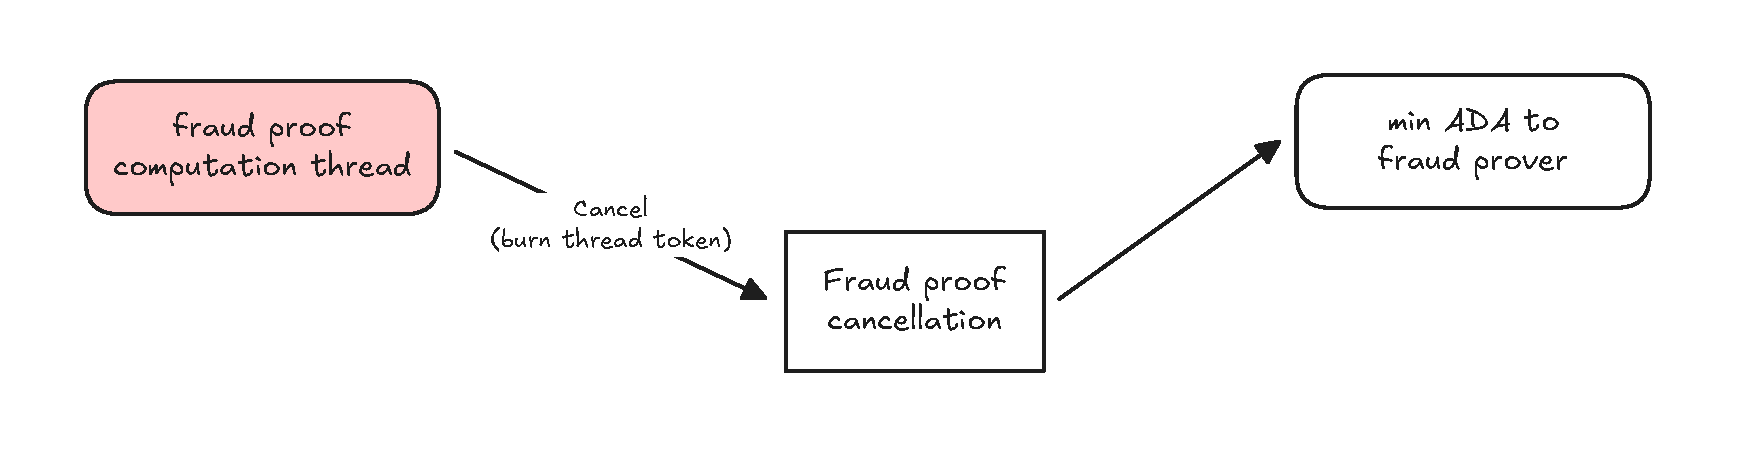
\includegraphics[width=\txDiagramScale\linewidth]{\subfix{../images/tx-diagram/O-fraud-proof-cancel.pdf}}
\end{center}
\caption[Fraud proof cancel]{Cancel the verification of a fraud proof.}
\label{fig:tx-fraud-proof-cancel}
\end{figure}

Cancel the verification of a fraud proof via a transaction that (\cref{fig:tx-fraud-proof-cancel}):
\begin{enumerate}
  \item Spends a single fraud proof computation thread utxo.
  \item Burns the computation thread token
  \item Refunds the ADA from the computation thread utxo to the fraud prover.
\end{enumerate}

Correctness is enforced by the Cancel redeemer of the fraud proof minting policy (\cref{h:fraud-proof-computation-threads-minting-policy}).

\begin{figure}[H]
\begin{center}
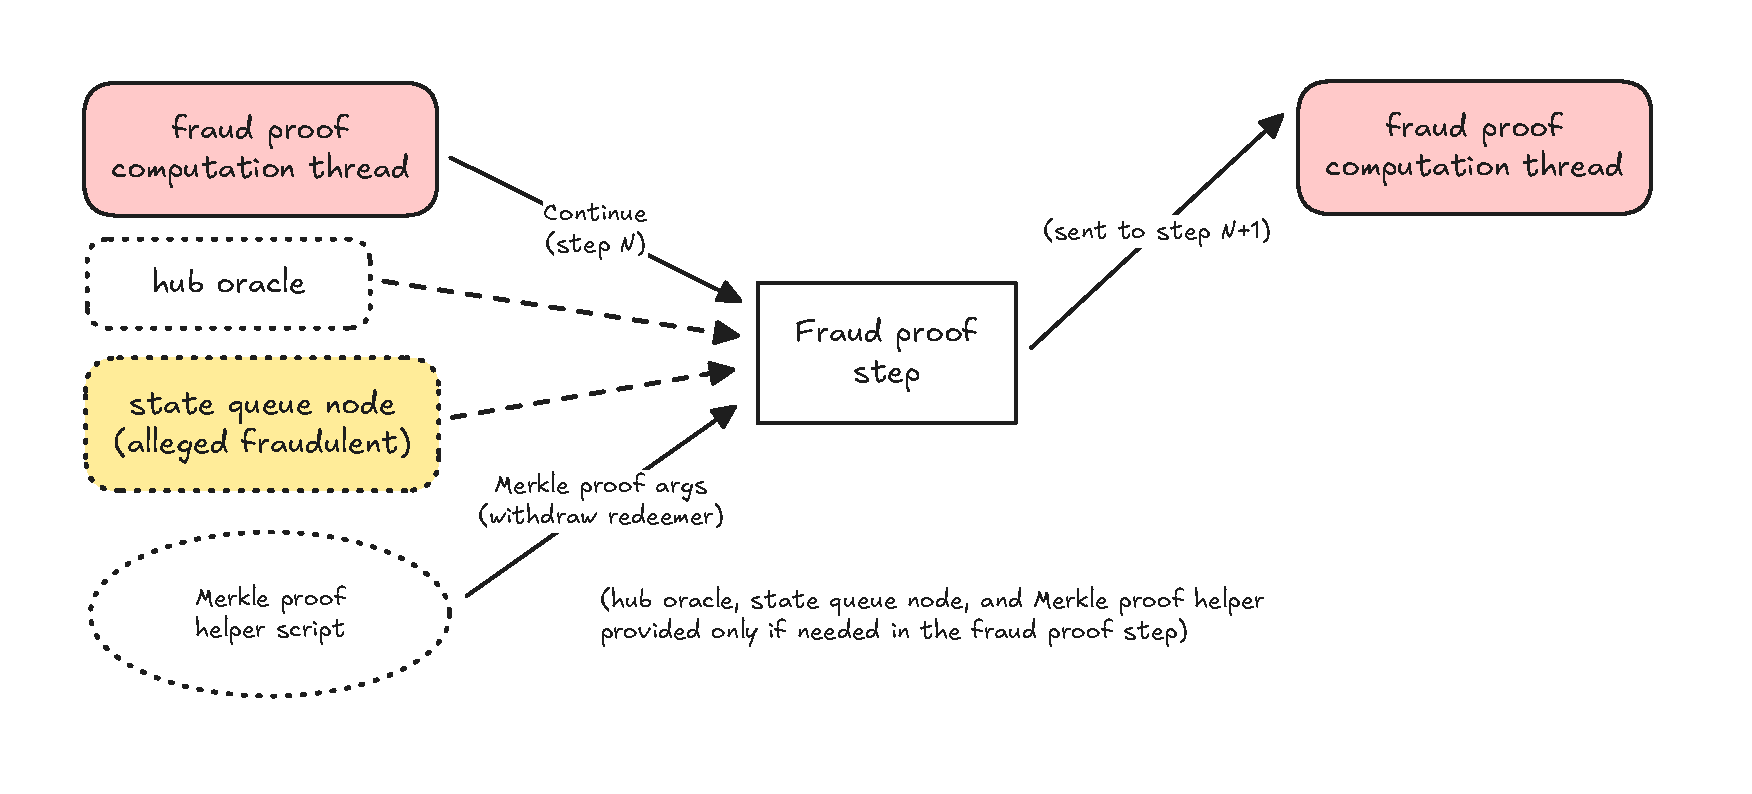
\includegraphics[width=\txDiagramScale\linewidth]{\subfix{../images/tx-diagram/P-fraud-proof-step.pdf}}
\end{center}
\caption[Fraud proof step]{Perform a verification step of a fraud proof.}
\label{fig:tx-fraud-proof-step}
\end{figure}

Perform a single verification step of a fraud proof via a transaction that (\cref{fig:tx-fraud-proof-step}):
\begin{enumerate}
  \item Spends a single fraud proof computation thread utxo, performing the verification step defined in the utxo's spending validator.
  \item Reproduces the fraud proof computation thread utxo as a continuing output sent to the next step's spending validator address.
  \item If required by the verification step, references the allegedly fraudulent state queue node.
  \item If required by the verification step, withdraws ADA from a designated account that triggers Midgard's Merkle proof helper script.
\end{enumerate}

Correctness is jointly enforced by these script redeemers:
\begin{itemize}
  \item Continue of the fraud proof's spending validator (\cref{h:fraud-proof-computation-threads-spending-validators}).
  \item (If needed) Merkle Inclusion/Exclusion Proof of the helper script staking validator (see the Aiken Merkle Patricia Forestry repository on Github).
\end{itemize}

\begin{figure}[H]
\begin{center}
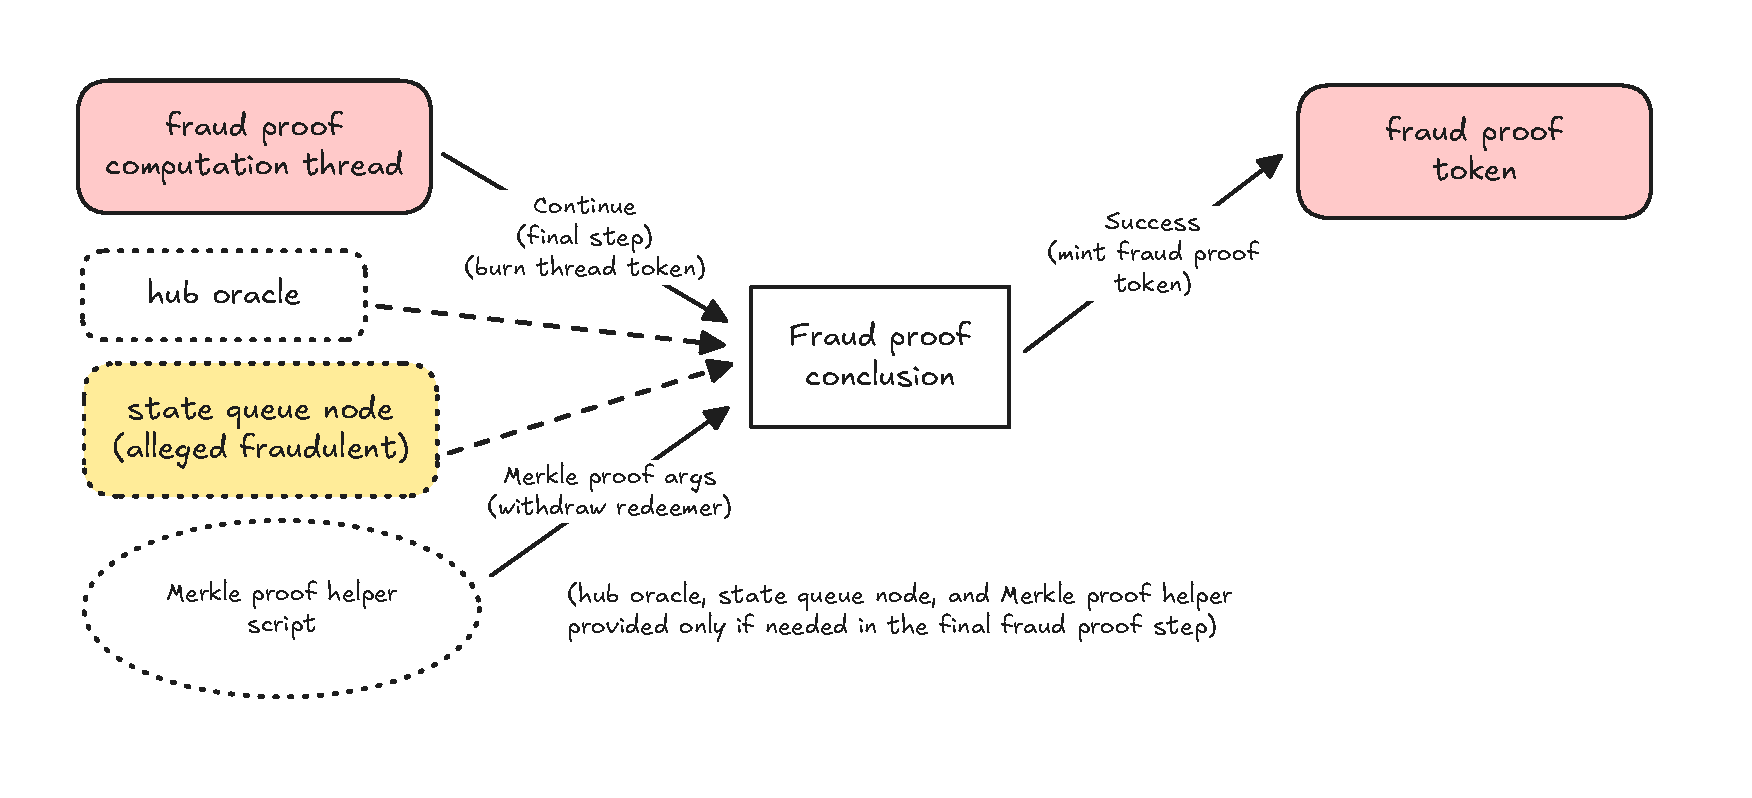
\includegraphics[width=\txDiagramScale\linewidth]{\subfix{../images/tx-diagram/Q-fraud-proof-conclude.pdf}}
\end{center}
\caption[Fraud proof conclude]{Conclude the verification of a fraud proof by performing its final step.}
\label{fig:tx-fraud-proof-conclude}
\end{figure}


Perform the final verification step of a fraud proof via a transaction that (\cref{fig:tx-fraud-proof-step}):
\begin{enumerate}
  \item Spends a single fraud proof computation thread utxo, performing the verification step defined in the utxo's spending validator.
  \item Burns the computation thread token and mints the corresponding fraud proof token.
  \item If required by the verification step, references the allegedly fraudulent state queue node.
  \item If required by the verification step, withdraws ADA from a designated account that triggers Midgard's Merkle proof helper script.
\end{enumerate}

Correctness is jointly enforced by these script redeemers:
\begin{itemize}
  \item Mint of the fraud proof minting policy (\cref{h:fraud-proof-tokens-minting-policy}).
  \item Conclude of the fraud proof's spending validator (\cref{h:fraud-proof-computation-threads-spending-validators}).
  \item (If needed) Merkle Inclusion/Exclusion Proof of the helper script staking validator (see the Aiken Merkle Patricia Forestry repository on Github).
\end{itemize}

\end{document}
